% Options for packages loaded elsewhere
\PassOptionsToPackage{unicode}{hyperref}
\PassOptionsToPackage{hyphens}{url}
%
\documentclass[
  oneside]{book}
\usepackage{amsmath,amssymb}
\usepackage{lmodern}
\usepackage{ifxetex,ifluatex}
\ifnum 0\ifxetex 1\fi\ifluatex 1\fi=0 % if pdftex
  \usepackage[T1]{fontenc}
  \usepackage[utf8]{inputenc}
  \usepackage{textcomp} % provide euro and other symbols
\else % if luatex or xetex
  \usepackage{unicode-math}
  \defaultfontfeatures{Scale=MatchLowercase}
  \defaultfontfeatures[\rmfamily]{Ligatures=TeX,Scale=1}
\fi
% Use upquote if available, for straight quotes in verbatim environments
\IfFileExists{upquote.sty}{\usepackage{upquote}}{}
\IfFileExists{microtype.sty}{% use microtype if available
  \usepackage[]{microtype}
  \UseMicrotypeSet[protrusion]{basicmath} % disable protrusion for tt fonts
}{}
\makeatletter
\@ifundefined{KOMAClassName}{% if non-KOMA class
  \IfFileExists{parskip.sty}{%
    \usepackage{parskip}
  }{% else
    \setlength{\parindent}{0pt}
    \setlength{\parskip}{6pt plus 2pt minus 1pt}}
}{% if KOMA class
  \KOMAoptions{parskip=half}}
\makeatother
\usepackage{xcolor}
\IfFileExists{xurl.sty}{\usepackage{xurl}}{} % add URL line breaks if available
\IfFileExists{bookmark.sty}{\usepackage{bookmark}}{\usepackage{hyperref}}
\hypersetup{
  pdftitle={A Handy Workbook for Research Methods \& Statistics},
  pdfauthor={Phil McAleer},
  hidelinks,
  pdfcreator={LaTeX via pandoc}}
\urlstyle{same} % disable monospaced font for URLs
\usepackage[margin=1in]{geometry}
\usepackage{color}
\usepackage{fancyvrb}
\newcommand{\VerbBar}{|}
\newcommand{\VERB}{\Verb[commandchars=\\\{\}]}
\DefineVerbatimEnvironment{Highlighting}{Verbatim}{commandchars=\\\{\}}
% Add ',fontsize=\small' for more characters per line
\usepackage{framed}
\definecolor{shadecolor}{RGB}{248,248,248}
\newenvironment{Shaded}{\begin{snugshade}}{\end{snugshade}}
\newcommand{\AlertTok}[1]{\textcolor[rgb]{0.94,0.16,0.16}{#1}}
\newcommand{\AnnotationTok}[1]{\textcolor[rgb]{0.56,0.35,0.01}{\textbf{\textit{#1}}}}
\newcommand{\AttributeTok}[1]{\textcolor[rgb]{0.77,0.63,0.00}{#1}}
\newcommand{\BaseNTok}[1]{\textcolor[rgb]{0.00,0.00,0.81}{#1}}
\newcommand{\BuiltInTok}[1]{#1}
\newcommand{\CharTok}[1]{\textcolor[rgb]{0.31,0.60,0.02}{#1}}
\newcommand{\CommentTok}[1]{\textcolor[rgb]{0.56,0.35,0.01}{\textit{#1}}}
\newcommand{\CommentVarTok}[1]{\textcolor[rgb]{0.56,0.35,0.01}{\textbf{\textit{#1}}}}
\newcommand{\ConstantTok}[1]{\textcolor[rgb]{0.00,0.00,0.00}{#1}}
\newcommand{\ControlFlowTok}[1]{\textcolor[rgb]{0.13,0.29,0.53}{\textbf{#1}}}
\newcommand{\DataTypeTok}[1]{\textcolor[rgb]{0.13,0.29,0.53}{#1}}
\newcommand{\DecValTok}[1]{\textcolor[rgb]{0.00,0.00,0.81}{#1}}
\newcommand{\DocumentationTok}[1]{\textcolor[rgb]{0.56,0.35,0.01}{\textbf{\textit{#1}}}}
\newcommand{\ErrorTok}[1]{\textcolor[rgb]{0.64,0.00,0.00}{\textbf{#1}}}
\newcommand{\ExtensionTok}[1]{#1}
\newcommand{\FloatTok}[1]{\textcolor[rgb]{0.00,0.00,0.81}{#1}}
\newcommand{\FunctionTok}[1]{\textcolor[rgb]{0.00,0.00,0.00}{#1}}
\newcommand{\ImportTok}[1]{#1}
\newcommand{\InformationTok}[1]{\textcolor[rgb]{0.56,0.35,0.01}{\textbf{\textit{#1}}}}
\newcommand{\KeywordTok}[1]{\textcolor[rgb]{0.13,0.29,0.53}{\textbf{#1}}}
\newcommand{\NormalTok}[1]{#1}
\newcommand{\OperatorTok}[1]{\textcolor[rgb]{0.81,0.36,0.00}{\textbf{#1}}}
\newcommand{\OtherTok}[1]{\textcolor[rgb]{0.56,0.35,0.01}{#1}}
\newcommand{\PreprocessorTok}[1]{\textcolor[rgb]{0.56,0.35,0.01}{\textit{#1}}}
\newcommand{\RegionMarkerTok}[1]{#1}
\newcommand{\SpecialCharTok}[1]{\textcolor[rgb]{0.00,0.00,0.00}{#1}}
\newcommand{\SpecialStringTok}[1]{\textcolor[rgb]{0.31,0.60,0.02}{#1}}
\newcommand{\StringTok}[1]{\textcolor[rgb]{0.31,0.60,0.02}{#1}}
\newcommand{\VariableTok}[1]{\textcolor[rgb]{0.00,0.00,0.00}{#1}}
\newcommand{\VerbatimStringTok}[1]{\textcolor[rgb]{0.31,0.60,0.02}{#1}}
\newcommand{\WarningTok}[1]{\textcolor[rgb]{0.56,0.35,0.01}{\textbf{\textit{#1}}}}
\usepackage{longtable,booktabs,array}
\usepackage{calc} % for calculating minipage widths
% Correct order of tables after \paragraph or \subparagraph
\usepackage{etoolbox}
\makeatletter
\patchcmd\longtable{\par}{\if@noskipsec\mbox{}\fi\par}{}{}
\makeatother
% Allow footnotes in longtable head/foot
\IfFileExists{footnotehyper.sty}{\usepackage{footnotehyper}}{\usepackage{footnote}}
\makesavenoteenv{longtable}
\usepackage{graphicx}
\makeatletter
\def\maxwidth{\ifdim\Gin@nat@width>\linewidth\linewidth\else\Gin@nat@width\fi}
\def\maxheight{\ifdim\Gin@nat@height>\textheight\textheight\else\Gin@nat@height\fi}
\makeatother
% Scale images if necessary, so that they will not overflow the page
% margins by default, and it is still possible to overwrite the defaults
% using explicit options in \includegraphics[width, height, ...]{}
\setkeys{Gin}{width=\maxwidth,height=\maxheight,keepaspectratio}
% Set default figure placement to htbp
\makeatletter
\def\fps@figure{htbp}
\makeatother
\setlength{\emergencystretch}{3em} % prevent overfull lines
\providecommand{\tightlist}{%
  \setlength{\itemsep}{0pt}\setlength{\parskip}{0pt}}
\setcounter{secnumdepth}{5}
\usepackage{booktabs}

\usepackage{tcolorbox}
\usepackage[T1]{fontenc}

\definecolor{dangcol}{RGB}{152,62,130}
\definecolor{warncol}{RGB}{245,220,112}
\definecolor{infocol}{RGB}{70,122,172}
\definecolor{trycol}{RGB}{97,88,156}

\newtcolorbox{dangerous}{
  colback=dangcol!10,
  colframe=dangcol,
  coltext=black,
  boxsep=5pt,
  arc=4pt
}

\newtcolorbox{warning}{
  colback=warncol!10,
  colframe=warncol,
  coltext=black,
  boxsep=5pt,
  arc=4pt
}

\newtcolorbox{info}{
  colback=infocol!10,
  colframe=infocol,
  coltext=black,
  boxsep=5pt,
  arc=4pt
}

\newtcolorbox{try}{
  colback=trycol!10,
  colframe=trycol,
  coltext=black,
  boxsep=5pt,
  arc=4pt
}
\ifluatex
  \usepackage{selnolig}  % disable illegal ligatures
\fi
\usepackage[]{natbib}
\bibliographystyle{plainnat}

\title{A Handy Workbook for Research Methods \& Statistics}
\author{Phil McAleer}
\date{Last Update: 2021-10-04}

\begin{document}
\maketitle

{
\setcounter{tocdepth}{1}
\tableofcontents
}
\hypertarget{overview}{%
\chapter*{Overview}\label{overview}}
\addcontentsline{toc}{chapter}{Overview}

\textbf{PLEASE NOTE THIS BOOK IS IN EARLY STAGES OF DEVELOPMENT AND WILL BE ADDED TO AND MAY VERY WELL CURRENTLY CONTAIN MISTAKES}

\textbf{Authors:} Phil McAleer

\textbf{Aim:} A Handy Workbook to help students understand Research Methods and Statistics through worked examples and self-tests.

\textbf{Contact:} This book is a living document and will be regularly checked and updated for improvements. Should you have any issues using the book or queries, please contact \href{mailto:philip.mcaleer@glasgow.ac.uk}{Phil McAleer}.

\textbf{R Version:} This book has been written with R version 4.1.1 (2021-08-10)

\textbf{Randomising Seed:} In chapters that use some level of randomisation, where we have remembered, the seed is set as 1409.

\hypertarget{foreword}{%
\chapter*{Foreword}\label{foreword}}
\addcontentsline{toc}{chapter}{Foreword}

This book is designed to help people understand the statistical tests commonly taught in a Psychology undergraduate course by walking through the tests in a step-by-step process. When we run analytical tests we often employ a statistical software to carry out the tests for us and our role, as researchers, is reduced to inputting the data in a corret format and interpreting the output. However, for us to understand and verify that the software is working correctly we must have some working knowledge of the test being used. For example, if a t-test comes back positive or negative, by understanding the processes involved in the calculation we can understand why that happens and what it means in terms of the research question we have set. Likewise, by understanding how degrees of freedom relate to different tests we can verify the output from the software, making sure that the values we get are appropriate. So whilst we, as researchers, will rarely have to run a full analysis by hand, and from memory, to fully understand the analyses that are the bases of the papers we write, it is important to know our way around those tests and how they work; it is unwise to just use an analytical software blindly without having some grasp of what it is doing and then using that output to make claims about human behavior. We hope that this book helps in that understanding and in turn improves your research practice. If you have any suggestions for improvements to this book or would like to see a test added, please do let us know!

\hypertarget{descriptives}{%
\chapter{Descriptives}\label{descriptives}}

\hypertarget{a-note-on-descriptives-and-inferentials}{%
\section{A note on Descriptives and Inferentials}\label{a-note-on-descriptives-and-inferentials}}

In the first part of this book we are going to look at descriptive statistics which we use to summarise and describe data we have collected - normally from a sample of the population of interest. Remember that the population is all the members of a group that we wish to generalise our findings to, and the sample is the subset of that population we have gathered data from. We draw our sample from the population, so to speak. The population is what we determine it to be based on our research question - everyone in Psychology at Glasgow; everyone study Psychology in Scotland; everyone studying Psychology in the world! Most of the time, testing everyone in a population is an unrealistic goal so we take a sample of that population and make inferences from that sample to the population using statistics. And the first step we take is to describe our sample.

Descriptive statistics can be broken down into three kinds:

\begin{itemize}
\tightlist
\item
  point estimates - these tend to be single values, or points, that summarise a set of data. Most common would be ones that summarise the center of the data such as the mean and the median.
\item
  interval estimates - these tend to be a range of values that summarise a set of data. Most common would be ones that summarise the spread of the data such as the variance and the standard deviation.
\item
  visualisations - are figures that help display the point and interval estimates of the data and can take various different forms depending on the data type.
\end{itemize}

Once we have described the data in our sample we then use inferential statistics to make predictions about, or comparisons between, our data. We infer how the general population would perform based on the sample we have collected and described. We will look at inferential statistics later in this book but first we will start with descriptives statistics, looking at point estimates first, before moving on to interval estimates.

\textbf{Point Estimates}

We will start by looking at three point estimates. They are:

\begin{itemize}
\tightlist
\item
  the Mean
\item
  the Median
\item
  the Mode
\end{itemize}

\hypertarget{the-mean}{%
\section{The Mean}\label{the-mean}}

The mean is a descriptive statistic that measures the average value of a set of numbers.

The symbol for the mean is generally written as \(\overline{X}\) (pronounced as X-bar) and the formula for the mean is:

\[\overline{X} = \frac{\sum_i^n{x_i}}{n}\]

Which reads as sum (\(\sum\)) all the values from \(i\) (the first value) to \(n\) (the last value) and then divide that number by the total number of values (\(n\)). Let's look at an example.

Say we are interested in how years of experience in driving impacts on some metric of peformance. We recruit 25 participants and ask them how many years they have been driving. Here are their responses:

If we start to fill in the information from above we get:

\[\overline{X} = \frac{7 +
1 +
2+
6+
3+\\
4+
3+
4+
3+
4+\\
5+
4+
7+
5+
6+\\
5+
5+
4+
5+
6+\\
5+
6+
3+
2+
5}{25}\]

So the first step is to add all the values on the top half of the formula together, which is called the numerator, giving us:

\[\overline{X} =\frac{110}{25}\]

Which can also be read as:

\[\overline{X} = 110/25\]

And if we then divide top of the formula, the numerator, by the bottom half, called the denominator, we would get:

\[\overline{X} = 4.4\]

And so, when using the standard APA write-up format of \textbf{M = \ldots{}}, we would write \textbf{M = 4.4}.

\hypertarget{the-median}{%
\section{The Median}\label{the-median}}

The median is the next point estimate we will look at and is the middle number in a distribution where half of the values in the data are larger and half are smaller. It is literally the value that divides the data in half.

The standard way of calculating the Median involves two steps:

\begin{enumerate}
\def\labelenumi{\arabic{enumi}.}
\tightlist
\item
  Sort all values from lowest to highest (i.e.~from \(i\) (the first value) to \(n\) (the last value))
\item
  The median is the value at position \(\frac{(n + 1)}{2}\)
\end{enumerate}

So if we look at our driving data again, the responses were:

\[7, 1, 2, 6, 3, 4, 3, 4, 3, 4, 5, 4, 7, 5, 6, 5, 5, 4, 5, 6, 5, 6, 3, 2, 5\]

And if we sort them from lowest value to highest value we get:

\[1, 2, 2, 3, 3, 3, 3, 4, 4, 4, 4, 4, 5, 5, 5, 5, 5, 5, 5, 6, 6, 6, 6, 7, 7\]

Now we need to figure out what the value would be at the median position of our dataset, where the median position is \(\frac{(n + 1)}{2}\) and we have n = 25 participants.

\[Median\space Position = \frac{(n + 1)}{2} = \frac{(25 + 1)}{2} = \frac{26}{2} = 13\]

Meaning that the Median Position for n = 25 is the 13\textsuperscript{th} position and so the Median is the value at position 13 after we have sorted the data from smallest to largest:

\[1, 2, 2, 3, 3, 3, 3, 4, 4, 4, 4, 4, 5, 5, 5, 5, 5, 5, 5, 6, 6, 6, 6, 7, 7\]

And if we count along the line until we get to the Median Position, we can see that the value in position 13 is 5, meaning that for this data the Median = 5. And so, when using the standard APA write-up format of \textbf{Mdn = \ldots{}}, we would write \textbf{Mdn = 5}.

\hypertarget{the-mode}{%
\section{The Mode}\label{the-mode}}

The mode is the last point estimate we will consider here and is the value or category that appears most often, most frequently, in your data set. There is no formula for the mode and it involves counting how many of each category or value you have and finding the most common one. Here are our values again:

\[7, 1, 2, 6, 3, 4, 3, 4, 3, 4, 5, 4, 7, 5, 6, 5, 5, 4, 5, 6, 5, 6, 3, 2, 5\]

And if we sort them from largest to smallest for easy of reading we get:

\[1, 2, 2, 3, 3, 3, 3, 4, 4, 4, 4, 4, 5, 5, 5, 5, 5, 5, 5, 6, 6, 6, 6, 7, 7\]

And if we start to count all the different values we see that we have:

Years

n

1

1

2

2

3

4

4

5

5

7

6

4

7

2

Meaning, for example, we have 4 people with three years of driving experience, and 5 people with four years of driving experience. And looking at our table we can see the most common number of years of driving experience is 5 as there are 7 with that number of years experience. We would therefore write \textbf{Mode = 5}

\hypertarget{section-glossary}{%
\subsection{Section glossary}\label{section-glossary}}

term

definition

denominator

name for the bottom half of a formula

descriptive

Statistics that describe an aspect of data (e.g., mean, median, mode, variance, range)

inferential

Statistics that allow you to make predictions about or comparisons between data (e.g., t-value, F-value, rho)

interval-estimates

a range of values that summarise an aspect of a data set. Examples include the range, variance, standard deviation, standard error and confidence intervals.

mean

A descriptive statistic that measures the average value of a set of numbers.

median

The middle number in a distribution where half of the values are larger and half are smaller.

numerator

name for the top half of a formula

participant

the word used to describe someone who has taken part in a study. Note that subject is outdated and no longer used.

point-estimates

a single value that summarises an aspect of a data set. Examples include the mean, median, and the mode.

population

All members of a group that we wish to generalise our findings to. E.g. all students taking Psychology at the University of Glasgow. We draw our testing sample from the population.

sample

A subset of the population that you wish to make an inference about through your test.

\hypertarget{a-full-desciptive-example}{%
\section{A full desciptive example}\label{a-full-desciptive-example}}

\textbf{The Data}

To look at a full descriptive example including the mean, variance, standard deviation, standard error, 95\% Confidence Intervals, and z-scores, we will use the following data from 10 participants:

Participants

X

1

8

2

11

3

6

4

3

5

1

6

6

7

1

8

0

9

1

10

4

\hypertarget{the-mean-1}{%
\subsection{The Mean}\label{the-mean-1}}

The symbol for the mean is generally written as \(\overline{X}\) (pronounced as X-bar) and the formula for the mean is:

\[\overline{X} = \frac{\sum_i^n{x_i}}{n}\]

Which reads as sum (\(\sum\)) all the values from \(i\) (the first value) to \(n\) (the last value) and then divide that number by the total number of values (\(n\)). If we start to fill in the information from above we get:

\[\overline{X} = \frac{8 + 11 + 6 +3 +1 +6 +1 +0 +1 +4}{10}\]

And if we sum all the values on the top half together we get:

\[\overline{X} = \frac{41}{10}\]

And finally divide the top half by the bottom half, leaving:

\[\overline{X} = 4.1\]

We find that the mean, rounded to two decimal places, is \textbf{\(\overline{X} = 4.1\)}

\hypertarget{variance}{%
\subsection{Variance}\label{variance}}

The symbol for the variance is generally written as \(s^2\) (pronounced as sigma-squared) but can also be written as \(Var\). The formula for the variance is:

\[s^2 = \frac{\sum_i^n(x_{i} - \overline{x})^2}{n-1}\]

So let's again start by filling in the numbers to the formula:

\[s^2 = \frac{(8 - 4.1)^2 + (11 - 4.1)^2 + (6 - 4.1)^2 + (3 - 4.1)^2 + (1 - 4.1)^2 + \\(6 - 4.1)^2 + (1 - 4.1)^2 + (0 - 4.1)^2 + (1 - 4.1)^2 + (4 - 4.1)^2}{10 - 1}\]

And we do the subtractions in all those brackets of the top half and the one on the bottom:

\[s^2 = \frac{(3.9)^2 + (6.9)^2 + (1.9)^2 + (-1.1)^2 + (-3.1)^2 + \\(1.9)^2 + (-3.1)^2 + (-4.1)^2 + (-3.1)^2 + (-0.1)^2}{9}\]

Then we square all those values on the top half:

\[s^2 = \frac{15.21 + 47.61+ 3.61+ 1.21+ 9.61+ 3.61+ 9.61+ 16.81+ 9.61+ 0.01}{9}\]

Sum those values together:

\[s^2 = \frac{116.9}{9}\]
And divide the top half by the bottom half:

\[s^2 = 12.9888889\]

Showing that the variance, rounded to two decimal places is, \textbf{\(s^2 = 12.99\)}

\hypertarget{standard-deviation}{%
\subsection{Standard Deviation}\label{standard-deviation}}

The symbol for the standard deviation is generally written as \(s\) (pronounced as sigma) but can also be written as \(SD\). The formula for the standard deviation is:

\[s = \sqrt\frac{\sum_i^n(x_{i} - \overline{x})^2}{n-1}\]
So let's again start by filling in the numbers to the formula:

\[s = \sqrt\frac{(8 - 4.1)^2 + (11 - 4.1)^2 + (6 - 4.1)^2 + (3 - 4.1)^2 + (1 - 4.1)^2 + \\(6 - 4.1)^2 + (1 - 4.1)^2 + (0 - 4.1)^2 + (1 - 4.1)^2 + (4 - 4.1)^2}{10 - 1}\]

And we do the subtractions in all those brackets of the top half and the one on the bottom:

\[s = \sqrt\frac{(3.9)^2 + (6.9)^2 + (1.9)^2 + (-1.1)^2 + (-3.1)^2 + \\(1.9)^2 + (-3.1)^2 + (-4.1)^2 + (-3.1)^2 + (-0.1)^2}{9}\]

Then we square all those values on the top half:

\[s = \sqrt\frac{15.21 + 47.61+ 3.61+ 1.21+ 9.61+ 3.61+ 9.61+ 16.81+ 9.61+ 0.01}{9}\]

Sum those values together:

\[s = \sqrt\frac{116.9}{9}\]
Divide the top half by the bottom half:

\[s = \sqrt{12.9888889}\]

And finally take the square root:

\[s = 3.6040101\]

We find that the standard deviation, rounded to two decimal places, is \textbf{\(s = 3.6\)}

\hypertarget{var-to-sd}{%
\subsection{Var to SD}\label{var-to-sd}}

Remembering that the standard deviation is the square root of the variance, then if you know the variance (\(s^2\)) and you need the standard deviation (\(s\)) then you can do:

\[s = \sqrt{s^2}\]

In our example, \(s^2 = 12.9888889\) and so

\[s = \sqrt{12.9888889}\]

giving:

\[s = 3.6040101\]

\hypertarget{sd-to-var}{%
\subsection{SD to Var}\label{sd-to-var}}

Sometimes you need to go from the standard deviation to the variance, and remembering that the variance is the standard deviation squared, or the standard deviation multiplied by itself, then you can do:

\[s^2 = s \times s\]

And if we know that the standard deviation in our example is \(s = 3.6040101\) then:

\[s^2 = 3.6040101 \times 3.6040101\]

giving us:

\[s^2 = 12.9888889\]

\hypertarget{z-scores}{%
\subsection{Z-Scores}\label{z-scores}}

Any value on a continuous scale can be converted to a z-score (standard deviation units) through the formula:

\[z = \frac{x - \overline{x}}{s_{x}}\]

which can be read as the value (\(x\)) minus the mean value of the data (\(\overline{x}\)), divided by the standard deviation of the data (\(s_{X}\)). For example, if we look at Participant 1:

\begin{itemize}
\tightlist
\item
  \(x = 8\)
\item
  \(\overline{x} = 4.1\)
\item
  \(s_{x} = 3.6040101\)
\end{itemize}

Which if we fill in the formula we get:

\[z = \frac{8 - 4.1}{3.6040101}\]

And if we sort our the top half first:

\[z = \frac{3.9}{3.6040101}\]

Leaving us with:

\[z = 1.0821279\]

So Participant 1, when converted to a z-score and rounded to two decimal places, would have \textbf{z = 1.08}

\hypertarget{standard-error-of-the-mean}{%
\subsection{Standard Error of the Mean}\label{standard-error-of-the-mean}}

The symbol for the standard error is usually \(SE\) but can also be written as \(SEM\) when specificaly about the mean - short for standard error of the mean. The formula for the standard error is the standard deviation (\(s\)) divided by the square root of the number of observations (\(\sqrt{n}\)), and is written as:

\[SE = \frac{s}{\sqrt{n}}\]

but can also be written as:

\[SE = \frac{SD}{\sqrt{n}}\]

We know that our \(SD = 3.6040101\) and that we have \(n = 10\) participants, so:

\[SE = \frac{3.6040101}{\sqrt{10}}\]

And if we do the square root of the bottom half (denominator):

\[SE = \frac{3.6040101}{3.1622777}\]

And divide the top by the bottom:

\[SE = 1.1396881\]

We find that the standard error, rounded to two decimal places, is \(SE = 1.14\)

\hypertarget{confidence-intervals}{%
\subsection{Confidence Intervals}\label{confidence-intervals}}

We will specifically focus on the 95\% Confidence Interval using the cut-off value (assuming \(\alpha = .05\) and two-tailed) of \(z = 1.96\). The key formulas are:

\[Upper \space 95\%CI = \overline{x} + (z \times SE)\]

And

\[Lower \space 95\%CI = \overline{X} - (z \times SE)\]

We know that:

\begin{itemize}
\tightlist
\item
  \(\overline{x} = 4.1\)
\item
  \(SE = 1.1396881\)
\item
  \(z = 1.96\)
\end{itemize}

\textbf{Upper 95\% CI}

Dealing with the \textbf{Upper 95\% CI} we get:

\[Upper \space 95\%CI = 4.1 + (1.96 \times 1.1396881)\]

And if we sort out the bracket first:

\[Upper \space 95\%CI = 4.1 + 2.2337886\]

Which leaves us with:

\[Upper \space 95\%CI = 6.3337886\]

\textbf{Lower 95\% CI}

And now the \textbf{Lower 95\% CI} we get:

\[Lower \space 95\%CI = 4.1 - (1.96 \times 1.1396881)\]

And if we sort out the bracket first:

\[Lower \space 95\%CI = 4.1 - 2.2337886\]

Which leaves us with:

\[Lower \space 95\%CI = 1.8662114\]

And if we round both those values to two decimal places, then you get \textbf{\(Lower \space 95\%CI = 1.87\)} and \textbf{\(Upper \space 95\%CI = 6.33\)}

\hypertarget{the-write-up}{%
\subsection{The Write-Up}\label{the-write-up}}

And if we were to do a decent presentation of this data, including a measure of central tendency (the mean), a measure of spread relating to the sample (the standard deviation), and a measure of spread relating to the population (the 95\% CI), then it would start as something like: \textbf{``We ran 10 participants (M = 4.1, SD = 3.6, 95\%CI = {[}1.87, 6.33{]})\ldots..''}

\hypertarget{one-sample-chi-square}{%
\chapter{One-Sample Chi-Square}\label{one-sample-chi-square}}

\hypertarget{the-worked-example}{%
\section{The Worked Example}\label{the-worked-example}}

Here is our data:

Values

A

B

C

D

Observed

4

5

8

15

And if we add on a column showing the total number of participants, adding all the numbers in the different conditions together, (i.e.~4 + 5 + 8 + 15 = 32), then we get:

Values

A

B

C

D

Total

Observed

4

5

8

15

32

Now the formula for the chi-square is:

\[\chi^2 = \sum\frac{(Observed - Expected)^2}{Expected}\]

The Expected values for each condition, in a one-sample chi-square assuming a uniform (equal) distribution is calculated by \(N \times \frac{1}{k}\) where \(k\) is the number of conditions and \(N\) is the total number of participants. This can also be written more straightforward as \(N/k\). That means that in our example the expected value in each condition would be:

\[Expected = \frac{N}{k} = \frac{32}{4} = 8\]

Let's now add those Expected values to our table which looks like:

Values

A

B

C

D

Total

Observed

4

5

8

15

32

Expected

8

8

8

8

32

We now have our data, let's start putting it into the formula, which we said was:

\[\chi^2 = \sum\frac{(Observed - Expected)^2}{Expected}\]

Which really means:

\[\chi^2 = \frac{(Observed_{A} - Expected_{A})^2}{Expected_{A}} + \frac{(Observed_{B} - Expected_{B})^2}{Expected_{B}} +  \frac{(Observed_{C} - Expected_{C})^2}{Expected_{C}} + \\ \frac{(Observed_{D} - Expected_{D})^2}{Expected_{D}}\]

So

\[\chi^2 = \frac{(4 - 8)^2}{8}+\frac{(5 - 8)^2}{8}+\frac{(8 - 8)^2}{8}+\frac{(15 - 8)^2}{8}\]

Which becomes:

\[\chi^2 = \frac{(-4)^2}{8} + \frac{(-3)^2}{8} + \frac{(0)^2}{8} + \frac{(7)^2}{8}\]

And if we now square the top halves (the numerators):

\[\chi^2 = \frac{16}{8} + \frac{9}{8} + \frac{0}{8} + \frac{49}{8}\]

Then divide the top half by the bottom half for each condition:

\[\chi^2 = {2}+{1.125}+{0}+{6.125}\]
And finally add them altogether

\[\chi^2 = 9.25\]

So we find that \(\chi^2 = 9.25\)

The degrees of freedom in this test is \(k - 1\) and given that we have 4 conditions:

\[df = k - 1\]
\[df = 4 - 1\]
\[df = 3\]

\textbf{The effect size}

A common effect size for the one-sample chi-square test is \(\phi\) (pronounced ``ph-aye'' and can be written as ``phi''). The formula for \(\phi\) is:

\[\phi = \sqrt\frac{\chi^2}{N}\]

And if we know that \(\chi^2 =9.25\) and that \(N = 32\), then putting them into the formula we get:

\[\phi = \sqrt\frac{9.25}{32}\]

\[\phi = 0.5376453\]

\textbf{The write-up}

If we were to look at a critical value look-up table, we would see that the critical value associated with a \(df = 3\) at \(\alpha = .05\), to three decimal places, is \(\chi^2_{crit} = 7.815\). As the chi-square value of this test (i.e.~\(\chi^2 = 9.25\)) is larger than \(\chi^2_{crit}\) then we can say that our test is significant, and as such would be written up as \(\chi^2(df = 3, N = 32) = 9.25,p < .05\).

Finally, if our test was significant then all we need to do is state the condition with the highest frequency (i.e.~the mode), which in this case is Condition D

\hypertarget{test-yourself}{%
\section{Test Yourself}\label{test-yourself}}

\hypertarget{dataset-1}{%
\subsection{DataSet 1}\label{dataset-1}}

Here is our data:

Values

A

B

C

D

Observed

6

0

1

11

Show me the working and answer

And if we add on a column showing the total number of participants, adding all the numbers in the different conditions together, (i.e.~6 + 0 + 1 + 11 = 18), then we get:

Values

A

B

C

D

Total

Observed

6

0

1

11

18

Now the formula for the chi-square is:

\[\chi^2 = \sum\frac{(Observed - Expected)^2}{Expected}\]

The Expected values for each condition, in a one-sample chi-square assuming a uniform (equal) distribution is calculated by \(N \times \frac{1}{k}\) where \(k\) is the number of conditions and \(N\) is the total number of participants. This can also be written more straightforward as \(N/k\). That means that in our example the expected value in each condition would be:

\[Expected = \frac{N}{k} = \frac{18}{4} = 4.5\]

Let's now add those Expected values to our table which looks like:

Values

A

B

C

D

Total

Observed

6.0

0.0

1.0

11.0

18

Expected

4.5

4.5

4.5

4.5

18

We now have our data, let's start putting it into the formula, which we said was:

\[\chi^2 = \sum\frac{(Observed - Expected)^2}{Expected}\]

So

\[\chi^2 = \frac{(6 - 4.5)^2}{4.5}+\frac{(0 - 4.5)^2}{4.5}+\frac{(1 - 4.5)^2}{4.5}+\frac{(11 - 4.5)^2}{4.5}\]

Which becomes:

\[\chi^2 = \frac{(1.5)^2}{4.5} + \frac{(-4.5)^2}{4.5} + \frac{(-3.5)^2}{4.5} + \frac{(6.5)^2}{4.5}\]

And if we now square the top halves (the numerators):

\[\chi^2 = \frac{2.25}{4.5} + \frac{20.25}{4.5} + \frac{12.25}{4.5} + \frac{42.25}{4.5}\]

Then divide the top half by the bottom half for each condition:

\[\chi^2 = {0.5}+{4.5}+{2.7222222}+{9.3888889}\]
And finally add them altogether

\[\chi^2 = 17.1111111\]

So we find that \(\chi^2 = 17.1111111\)

The degrees of freedom in this test is \(k - 1\) and given that we have 4 conditions:

\[df = k - 1\]
\[df = 4 - 1\]
\[df = 3\]

\textbf{The effect size}

A common effect size for the one-sample chi-square test is \(\phi\) (pronounced ``ph-aye'' and can be written as ``phi''). The formula for \(\phi\) is:

\[\phi = \sqrt\frac{\chi^2}{N}\]

And if we know that \(\chi^2 =17.1111111\) and that \(N = 18\), then putting them into the formula we get:

\[\phi = \sqrt\frac{17.1111111}{18}\]

\[\phi = 0.974996\]

\textbf{The write-up}

If we were to look at a critical value look-up table, we would see that the critical value associated with a \(df = 3\) at \(\alpha = .05\), to three decimal places, is \(\chi^2_{crit} = 7.815\). As the chi-square value of this test (i.e.~\(\chi^2 = 17.1111111\)) is larger than \(\chi^2_{crit}\) then we can say that our test is significant, and as such would be written up as \(\chi^2(df = 3, N = 18) = 17.1111111,p < .05\).

Finally, if our test was significant then all we need to do is state the condition with the highest frequency (i.e.~the mode), which in this case is Condition D

\hypertarget{dataset-2}{%
\subsection{DataSet 2}\label{dataset-2}}

Here is our data:

Values

A

B

C

D

Observed

12

16

11

14

Show me the working and answer

And if we add on a column showing the total number of participants, adding all the numbers in the different conditions together, (i.e.~12 + 16 + 11 + 14 = 53), then we get:

Values

A

B

C

D

Total

Observed

12

16

11

14

53

Now the formula for the chi-square is:

\[\chi^2 = \sum\frac{(Observed - Expected)^2}{Expected}\]

The Expected values for each condition, in a one-sample chi-square assuming a uniform (equal) distribution is calculated by \(N \times \frac{1}{k}\) where \(k\) is the number of conditions and \(N\) is the total number of participants. This can also be written more straightforward as \(N/k\). That means that in our example the expected value in each condition would be:

\[Expected = \frac{N}{k} = \frac{53}{4} = 13.25\]

Let's now add those Expected values to our table which looks like:

Values

A

B

C

D

Total

Observed

12.00

16.00

11.00

14.00

53

Expected

13.25

13.25

13.25

13.25

53

We now have our data, let's start putting it into the formula, which we said was:

\[\chi^2 = \sum\frac{(Observed - Expected)^2}{Expected}\]

So

\[\chi^2 = \frac{(12 - 13.25)^2}{13.25}+\frac{(16 - 13.25)^2}{13.25}+\frac{(11 - 13.25)^2}{13.25}+\frac{(14 - 13.25)^2}{13.25}\]

Which becomes:

\[\chi^2 = \frac{(-1.25)^2}{13.25} + \frac{(2.75)^2}{13.25} + \frac{(-2.25)^2}{13.25} + \frac{(0.75)^2}{13.25}\]

And if we now square the top halves (the numerators):

\[\chi^2 = \frac{1.5625}{13.25} + \frac{7.5625}{13.25} + \frac{5.0625}{13.25} + \frac{0.5625}{13.25}\]

Then divide the top half by the bottom half for each condition:

\[\chi^2 = {0.1179245}+{0.5707547}+{0.3820755}+{0.0424528}\]
And finally add them altogether

\[\chi^2 = 1.1132075\]

So we find that \(\chi^2 = 1.1132075\)

The degrees of freedom in this test is \(k - 1\) and given that we have 4 conditions:

\[df = k - 1\]
\[df = 4 - 1\]
\[df = 3\]

\textbf{The effect size}

A common effect size for the one-sample chi-square test is \(\phi\) (pronounced ``ph-aye'' and can be written as ``phi''). The formula for \(\phi\) is:

\[\phi = \sqrt\frac{\chi^2}{N}\]

And if we know that \(\chi^2 =1.1132075\) and that \(N = 53\), then putting them into the formula we get:

\[\phi = \sqrt\frac{1.1132075}{53}\]

\[\phi = 0.1449273\]

\textbf{The write-up}

If we were to look at a critical value look-up table, we would see that the critical value associated with a \(df = 3\) at \(\alpha = .05\), to three decimal places, is \(\chi^2_{crit} = 7.815\). As the chi-square value of this test (i.e.~\(\chi^2 = 1.1132075\)) is smaller than \(\chi^2_{crit}\) then we can say that our test is non-significant, and as such would be written up as \(\chi^2(df = 3, N = 53) = 1.1132075,p > .05\).

Finally, if our test was significant then all we need to do is state the condition with the highest frequency (i.e.~the mode), which in this case is Condition B

\hypertarget{dataset-3}{%
\subsection{DataSet 3}\label{dataset-3}}

Here is our data:

Values

A

B

C

D

Observed

20

9

19

1

Show me the working and answer

And if we add on a column showing the total number of participants, adding all the numbers in the different conditions together, (i.e.~20 + 9 + 19 + 1 = 49), then we get:

Values

A

B

C

D

Total

Observed

20

9

19

1

49

Now the formula for the chi-square is:

\[\chi^2 = \sum\frac{(Observed - Expected)^2}{Expected}\]

The Expected values for each condition, in a one-sample chi-square assuming a uniform (equal) distribution is calculated by \(N \times \frac{1}{k}\) where \(k\) is the number of conditions and \(N\) is the total number of participants. This can also be written more straightforward as \(N/k\). That means that in our example the expected value in each condition would be:

\[Expected = \frac{N}{k} = \frac{49}{4} = 12.25\]

Let's now add those Expected values to our table which looks like:

Values

A

B

C

D

Total

Observed

20.00

9.00

19.00

1.00

49

Expected

12.25

12.25

12.25

12.25

49

We now have our data, let's start putting it into the formula, which we said was:

\[\chi^2 = \sum\frac{(Observed - Expected)^2}{Expected}\]

So

\[\chi^2 = \frac{(20 - 12.25)^2}{12.25}+\frac{(9 - 12.25)^2}{12.25}+\frac{(19 - 12.25)^2}{12.25}+\frac{(1 - 12.25)^2}{12.25}\]

Which becomes:

\[\chi^2 = \frac{(7.75)^2}{12.25} + \frac{(-3.25)^2}{12.25} + \frac{(6.75)^2}{12.25} + \frac{(-11.25)^2}{12.25}\]

And if we now square the top halves (the numerators):

\[\chi^2 = \frac{60.0625}{12.25} + \frac{10.5625}{12.25} + \frac{45.5625}{12.25} + \frac{126.5625}{12.25}\]

Then divide the top half by the bottom half for each condition:

\[\chi^2 = {4.9030612}+{0.8622449}+{3.7193878}+{10.3316327}\]
And finally add them altogether

\[\chi^2 = 19.8163265\]

So we find that \(\chi^2 = 19.8163265\)

The degrees of freedom in this test is \(k - 1\) and given that we have 4 conditions:

\[df = k - 1\]
\[df = 4 - 1\]
\[df = 3\]

\textbf{The effect size}

A common effect size for the one-sample chi-square test is \(\phi\) (pronounced ``ph-aye'' and can be written as ``phi''). The formula for \(\phi\) is:

\[\phi = \sqrt\frac{\chi^2}{N}\]

And if we know that \(\chi^2 =19.8163265\) and that \(N = 49\), then putting them into the formula we get:

\[\phi = \sqrt\frac{19.8163265}{49}\]

\[\phi = 0.6359362\]

\textbf{The write-up}

If we were to look at a critical value look-up table, we would see that the critical value associated with a \(df = 3\) at \(\alpha = .05\), to three decimal places, is \(\chi^2_{crit} = 7.815\). As the chi-square value of this test (i.e.~\(\chi^2 = 19.8163265\)) is larger than \(\chi^2_{crit}\) then we can say that our test is significant, and as such would be written up as \(\chi^2(df = 3, N = 49) = 19.8163265,p < .05\).

Finally, if our test was significant then all we need to do is state the condition with the highest frequency (i.e.~the mode), which in this case is Condition A

\hypertarget{chisquare-look-up-table}{%
\section{ChiSquare Look-up Table}\label{chisquare-look-up-table}}

\begin{longtable}[]{@{}cc@{}}
\toprule
df & \(\alpha = .05\) \\
\midrule
\endhead
1 & 3.841 \\
2 & 5.991 \\
3 & 7.815 \\
4 & 9.488 \\
5 & 11.07 \\
6 & 12.592 \\
7 & 14.067 \\
8 & 15.507 \\
9 & 16.919 \\
10 & 18.307 \\
\bottomrule
\end{longtable}

\hypertarget{chi-square-cross-tabulation}{%
\chapter{Chi-Square Cross-Tabulation}\label{chi-square-cross-tabulation}}

\hypertarget{the-worked-example-1}{%
\section{The Worked Example}\label{the-worked-example-1}}

Here is our data:

Groups

Yes

No

A

88

93

B

160

59

We are going to need to know the Column Totals and Row Totals and the Total number of participants (N), so lets calculate them add them to our tables:

\begin{itemize}
\tightlist
\item
  \textbf{Group A Row Total} = 88 + 93 = 181
\item
  \textbf{Group B Row Total} = 160 + 59 = 219
\item
  \textbf{Yes Column Total} = 88 + 160 = 248
\item
  \textbf{No Column Total} = 93 + 59 = 152
\item
  \textbf{N =} 88 + 93 +160 + 59 = 400
\end{itemize}

And if we add those to our table we see:

Groups

Yes

No

Totals

A

88

93

181

B

160

59

219

Totals

248

152

400

Now the formula for the chi-square is:

\[\chi^2 = \sum\frac{(Observed - Expected)^2}{Expected}\]

The Expected values for each condition, in the cross-tabulation in a few ways but the one we will use here is probably the easiest to use and it is:

\[Expected = \frac{Total_{row} \times Total_{column}}{N_{total}}\]

This is the same as other versions you might have seen such as:

\[Expected = \frac{Total_{row}}{N_{total}} \times \frac{Total_{column}}{N_{total}} \times N_{total}\]

The will both give the same result. So using the first approach we would see that the Expected values are:

\textbf{For Group A people that said Yes:}

\[Expected_{A-Yes} = \frac{181 \times 248}{400} = \frac{44888}{400} = 112.22\]

\textbf{For Group A people that said No:}

\[Expected_{A-No} = \frac{181 \times 152}{400} = \frac{27512}{400} = 68.78\]

\textbf{For Group B people that said Yes:}

\[Expected_{B-Yes} = \frac{219 \times 248}{400} = \frac{54312}{400} = 135.78\]

\textbf{For Group B people that said No:}

\[Expected_{B-No} = \frac{219 \times 152}{400} = \frac{33288}{400} = 83.22\]

We now have our data, let's start putting it into the formula, which we said was:

\[\chi^2 = \sum\frac{(Observed - Expected)^2}{Expected}\]

Which really means:

\[\chi^2 = \frac{(Observed_{A-Yes} - Expected_{A-Yes})^2}{Expected_{A-Yes}} + \frac{(Observed_{A-No} - Expected_{A-No})^2}{Expected_{A-No}} + \\ \frac{(Observed_{B-Yes} - Expected_{B-Yes})^2}{Expected_{B-Yes}} +  \frac{(Observed_{B-No} - Expected_{B-No})^2}{Expected_{B-No}}\]

And if we start putting in the values, becomes:

\[\chi^2 = \frac{(88 - 112.22)^2}{112.22}+ \frac{(93 - 68.78)^2}{68.78}+\frac{(160 - 135.78)^2}{135.78}+\frac{(59 - 83.22)^2}{83.22}\]

And if we start to tidy those top halves up a little it becomes:

\[\chi^2 = \frac{(-24.22)^2}{112.22}+ \frac{(24.22)^2}{68.78}+\frac{(24.22)^2}{135.78}+\frac{(-24.22)^2}{83.22}\]

And now we square those top halves to give:

\[\chi^2 = \frac{586.6084}{112.22} + \frac{586.6084}{68.78} + \frac{586.6084}{135.78} + \frac{586.6084}{83.22} \]

And then divide the top halves by the bottom halves

\[\chi^2 = {5.2273071} + {8.5287642} + {4.3202858} + {7.0488873}\]

And then we sum them altogether to find:

\[\chi^2 = 25.1252443 \]

Meaning that, rounded to two decimal places, we find \(\chi^2 = 25.13\)

\textbf{Degrees of Freedom}

The degrees of freedom for the cross-tabulation is calculated as:

\[df = (Rows - 1) \times (Columns - 1)\]

Which is read as \textbf{the number of Rows minus 1 times the number of Columns minus 1}. If we look at our original data again:

Groups

Yes

No

A

88

93

B

160

59

Looking at the table we see we have 2 rows and 2 columns of actual observed data (not looking at the titles and group names), so:

\[Rows - 1 = 2 - 1 = 1\]

And

\[Columns - 1 = 2 - 1 = 1\]

Meaning that:

\[df = (Rows - 1) \times (Columns - 1)\]

which becomes:

\[df = (2 - 1) \times (2 - 1)\]

And reduces to:

\[df = (1) \times (1)\]

leaving us with:

\[df = 1\]

so we see that \(df = 1\)

\textbf{The effect size}

One of the common effect sizes for a cross-tabulation chi-square test is Cramer's \(V\) and is calculated as:

\[V = \sqrt\frac{\chi^2}{N \times \min(C-1, R-1)}\]

The key thing to note is \(\min(C-1, R-1)\) which is read as \textbf{the minimum of EITHER the number of Columns (C) minus 1 OR the number of Rows (R) minus 1}; whichever of those two values is smallest.

And the minimum of Columns minus 1 or Rows minus 1 is:

\[\min(C-1, R-1) = \min( 2 - 1,  2 - 1)\]
\[\min(C-1, R-1) = \min( 1,  1)\]
which gives us:

\[\min(C-1, R-1) = 1\]

And now we can start completing the Cramer's \(V\) formula as we know:

\begin{itemize}
\tightlist
\item
  \(\chi^2 = 25.13\)
\item
  \(N = 400\)
\item
  \(\min(C-1, R-1) = 1\)
\end{itemize}

Giving us:

\[V = \sqrt\frac{25.13}{400 \times 1}\]

And if we deal with the bottom half first we get:

\[V = \sqrt\frac{25.13}{400}\]

Then if we divide the top by the bottom we get

\[V = \sqrt{0.062825}\]

Giving us:

\[V = 0.2506492\]

So we see that, rounded to two decimal places, the effect size is \(V = 0.25\)

\textbf{The write-up}

If we were to look at a critical value look-up table, we would see that the critical value associated with a \(df = 1\) at \(\alpha = .05\), to three decimal places, is \(\chi^2_{crit} = 3.841\). As the chi-square value of this test (i.e.~\(\chi^2 = 25.13\)) is larger than \(\chi^2_{crit}\) then we can say that our test is significant, and as such would be written up as \(\chi^2(df = 1, N = 400) = 25.13,p < .05, V = 0.25\).

If our test was significant then we would go on to carry out the relevant one-sample chi-squares to breakdown how the association manifests itself. The key thing to remember however is that in these one-sample chi-squares, following the cross-tabulation, you \textbf{MUST} use the expected values from the cross-tabulation and \textbf{do not} calculate new expected values. For instance if you were looking at the one-sample chi-square within Group A, then you would use the expected values of \(Expected_{A-Yes} = 112.22\) and \(Expected_{A-No} = 68.78\) to compare against the observed values of \(Observed_{A-Yes} = 88\) and \(Observed_{A-No} = 93\) as such:

\[\chi^2 = \frac{(88 - 112.22)^2}{112.22}+ \frac{(93 - 68.78)^2}{68.78}\]

Which if you walk the process through you find:

\[\chi^2 = 13.7560713\]

Meaning that, rounded to two decimal places, we find \(\chi^2 = 13.76\)

\textbf{To Be Continued}

\hypertarget{test-yourself-1}{%
\section{Test Yourself}\label{test-yourself-1}}

\hypertarget{dataset-1-1}{%
\subsection{DataSet 1}\label{dataset-1-1}}

To Be Added

\hypertarget{chisquare-look-up-table-1}{%
\section{ChiSquare Look-up Table}\label{chisquare-look-up-table-1}}

\begin{longtable}[]{@{}cc@{}}
\toprule
df & \(\alpha = .05\) \\
\midrule
\endhead
1 & 3.841 \\
2 & 5.991 \\
3 & 7.815 \\
4 & 9.488 \\
5 & 11.07 \\
6 & 12.592 \\
7 & 14.067 \\
8 & 15.507 \\
9 & 16.919 \\
10 & 18.307 \\
\bottomrule
\end{longtable}

\hypertarget{between-subjects-students-t-test}{%
\chapter{Between-Subjects Student's t-test}\label{between-subjects-students-t-test}}

\textbf{between-subjects t-test:} Compare two groups or conditions where the participants are different in each group and have not been matched or are only matched on broad demographics, e.g.~only age.

\hypertarget{the-worked-example-2}{%
\section{The Worked Example}\label{the-worked-example-2}}

Here is your data:

Group

N

Mean

SD

A

18

25.58

2.25

B

18

29.07

2.53

Let's look at the main t-test formula:

\[t = \frac{\bar{X}_1 - \bar{X}_2}{s_p \times \sqrt{\frac{1}{N_1} + \frac{1}{N_2}}}\]

Now, from the table above we know:

\begin{itemize}
\tightlist
\item
  the mean of Group A is \(\bar{X_1} = 25.58\),
\item
  the mean of Group B is \(\bar{X_2} = 29.07\),
\item
  the N of Group A is \(N_1 = 18\),
\item
  and the N of Group B is \(N_2 = 18\),
\end{itemize}

which we can put into the equation right now:

\[t = \frac{25.58 - 29.07}{s_p \times \sqrt{\frac{1}{18} + \frac{1}{18}}}\]

And now we can see that the only thing we don't yet know is the pooled standard deviation (\(s_p\)). Let's look at that formula:

\textbf{Calculating the pooled standard deviation}

\[s_p = \sqrt{\frac{(n_1 -1)  \times s^2_{X_1} + (n_2 -1)\times s^2_{X_2}}{n_1 + n_2 - 2}}\]

And if we start to fill in some details:

\[s_p = \sqrt{\frac{(18 -1)  \times s^2_{X_1} + (18 -1)\times s^2_{X_2}}{18 + 18 - 2}}\]

Now looking at the formula, it is clear we are missing:

\begin{itemize}
\tightlist
\item
  \(s^2_{X_1}\) - the variance of Group A (could be written as \(s^2_{A}\))
\item
  \(s^2_{X_2}\) - the variance of Group B (could be written as \(s^2_{B}\))
\end{itemize}

What we do know though, from the table, is the standard deviations of both groups (\(SD_A\) = 2.25; \(SD_B\) = 2.53), and we know that variance of a group is equal to the standard deviation squared. So:

\begin{itemize}
\tightlist
\item
  \(s^2_{X_1}\) = \(s^2_A\) = \(SD_A \times SD_A\) = \(2.25 \times 2.25\) = \(5.0625\)
\item
  \(s^2_{X_2}\) = \(s^2_B\) = \(SD_B \times SD_B\) = \(2.53 \times 2.53\) = \(6.4009\)
\end{itemize}

And if we now add those values to our formula we get:

\[s_p = \sqrt{\frac{(18 -1)  \times 5.0625 + (18 -1)\times 6.4009}{18 + 18 - 2}}\]

And we can then start working through the formula, taking each stage in turn to make sure we don't make mistakes. Let's get rid of the brackets first:

\[s_p = \sqrt{\frac{(17  \times 5.0625) + (17 \times 6.4009)}{34}}\]

Now we deal with the multiplications:

\[s_p = \sqrt{\frac{86.0625 + 108.8153}{34}}\]

Let's tidy up that top half of the equation (the numerator):

\[s_p = \sqrt{\frac{194.8778}{34}}\]

Which if we then divide the numerator by the denominator (the bottom half), and then take the square root of that we get:

\[s_p = \sqrt{5.7317}\]

Giving a pooled standard deviation of:

\[s_p = 2.3940969\]

Meaning that our pooled standard deviation, rounded to three decimal places, is \(s_p = 2.394\) and we can now add that to the t-test formula to give us:

\textbf{Calculating the t-value}

\[t = \frac{25.58 - 29.07}{2.394 \times \sqrt{\frac{1}{18} + \frac{1}{18}}}\]

And again we just start working through the formula. Let's deal with the fractions relating to sample size first:

\[t = \frac{25.58 - 29.07}{2.394 \times \sqrt{0.0555556 + 0.0555556}}\]

Which we can tidy up a little to give:

\[t = \frac{-3.49}{2.394 \times \sqrt{0.1111111}}\]

And if we sort out the square root on the denominator we are left with:

\[t = \frac{-3.49}{2.394 \times 0.3333333}\]

We can then tidy up the denominator to give us:

\[t = \frac{-3.49}{0.798}\]

Which we can finally solve to give us a t-value, rounded to two decimal places, of \(t = -4.37\)

\textbf{Degrees of Freedom}

Great! Now we just need the degrees of freedom where the formula is:

\[df = (n_1 - 1) + (n_2 - 1)\]

And we already know that:

\begin{itemize}
\tightlist
\item
  the N of Group A is \(N_1 = 18\),
\item
  and the N of Group B is \(N_2 = 18\),
\end{itemize}

So putting them into the equation we get:

\[df = (18 - 1) + (18 - 1)\]
\[df = 17 + 17\]
\[df = 34\]

\textbf{Effect Size: Cohen's d}

And finally Cohen's d, the effect size:

\[d = \frac{2t}{\sqrt{df}}\]

Which, based on the info above, we know:

\begin{itemize}
\tightlist
\item
  \(t = -4.37\)
\item
  \(df = 34\)
\end{itemize}

Putting them into the formula we get:

\[d = \frac{2 \times -4.37}{\sqrt{34}}\]

And if we tidy the nominator and the denominator we get:

\[d = \frac{-8.74}{5.8309519}\]

Which we can then solve to learn that \(d = -1.5\)

\textbf{Determining Significance}

If we were to look at a critical values look-up table for \(df = 34\) and \(\alpha = .05\) (two-tailed), we would see that the critical value is \(t_{crit} = 2.032\). Given that our t-value, ignoring polarity and just looking at the absolute value, so \(t = 4.37\), is equal to or larger than our \(t_{crit}\) then we can say our result is significant, and as such would be written up as t(34) = 4.37, p \textless{} .05, d = 1.5

\textbf{Remember:} If you were writing this up as a report, and analysis the data in R, then you would see the p-value was actually p = \ensuremath{1.1081944\times 10^{-4}}, and would be written up as p \textless{} .001

\hypertarget{test-yourself-2}{%
\section{Test Yourself}\label{test-yourself-2}}

\hypertarget{dataset-1-2}{%
\subsection{DataSet 1}\label{dataset-1-2}}

Here is your data:

Group

N

Mean

SD

A

5

68.01

0.34

B

5

67.80

0.67

Show me the working and answer

Let's look at the main t-test formula:

\[t = \frac{\bar{X}_1 - \bar{X}_2}{s_p \times \sqrt{\frac{1}{N_1} + \frac{1}{N_2}}}\]

Now, from the table above we know:

\begin{itemize}
\tightlist
\item
  the mean of Group A is \(\bar{X_1} = 68.01\),
\item
  the mean of Group B is \(\bar{X_2} = 67.8\),
\item
  the N of Group A is \(N_1 = 5\),
\item
  and the N of Group B is \(N_2 = 5\),
\end{itemize}

which we can put into the equation right now:

\[t = \frac{68.01 - 67.8}{s_p \times \sqrt{\frac{1}{5} + \frac{1}{5}}}\]

And now we can see that the only thing we don't yet know is the pooled standard deviation (\(s_p\)). Let's look at that formula:

\[s_p = \sqrt{\frac{(n_1 -1)  \times s^2_{X_1} + (n_2 -1)\times s^2_{X_2}}{n_1 + n_2 - 2}}\]

And if we start to fill in some details:

\[s_p = \sqrt{\frac{(5 -1)  \times s^2_{X_1} + (5 -1)\times s^2_{X_2}}{5 + 5 - 2}}\]

Now looking at the formula, it is clear we are missing:

\begin{itemize}
\tightlist
\item
  \(s^2_{X_1}\) - the variance of Group A (could be written as \(s^2_{A}\))
\item
  \(s^2_{X_2}\) - the variance of Group B (could be written as \(s^2_{B}\))
\end{itemize}

What we do know though, from the table, is the standard deviations of both groups (\(SD_A\) = 0.34; \(SD_B\) = 0.67), and we know that variance of a group is equal to the standard deviation squared. So:

\begin{itemize}
\tightlist
\item
  \(s^2_{X_1}\) = \(s^2_A\) = \(SD_A \times SD_A\) = \(0.34 \times 0.34\) = \(0.1156\)
\item
  \(s^2_{X_2}\) = \(s^2_B\) = \(SD_B \times SD_B\) = \(0.67 \times 0.67\) = \(0.4489\)
\end{itemize}

And if we now add those values to our formula we get:

\[s_p = \sqrt{\frac{(5 -1)  \times 0.1156 + (5 -1)\times 0.4489}{5 + 5 - 2}}\]

And we can then start working through the formula, taking each stage in turn to make sure we don't make mistakes. Let's get rid of the brackets first:

\[s_p = \sqrt{\frac{(4  \times 0.1156) + (4 \times 0.4489)}{8}}\]

Now we deal with the multiplications:

\[s_p = \sqrt{\frac{0.4624 + 1.7956}{8}}\]

Let's tidy up that top half of the equation (the numerator):

\[s_p = \sqrt{\frac{2.258}{8}}\]

Which if we then divide the numerator by the denominator (the bottom half), and then take the square root of that we get:

\[s_p = \sqrt{0.28225}\]

Giving a pooled standard deviation of:

\[s_p = 0.5312721\]

Meaning that our pooled standard deviation, rounded to three decimal places, is \(s_p = 0.531\) and we can now add that to the t-test formula to give us:

\[t = \frac{68.01 - 67.8}{0.531 \times \sqrt{\frac{1}{5} + \frac{1}{5}}}\]

And again we just start working through the formula. Let's deal with the fractions relating to sample size first:

\[t = \frac{68.01 - 67.8}{0.531 \times \sqrt{0.2 + 0.2}}\]

Which we can tidy up a little to give:

\[t = \frac{0.21}{0.531 \times \sqrt{0.4}}\]

And if we sort out the square root on the denominator we are left with:

\[t = \frac{0.21}{0.531 \times 0.6324555}\]

We can then tidy up the denominator to give us:

\[t = \frac{0.21}{0.3358339}\]

Which we can finally solve to give us a t-value, rounded to two decimal places, of \(t = 0.63\)

Great! Now we just need the degrees of freedom where the formula is:

\[df = (n_1 - 1) + (n_2 - 1)\]

And we already know that:

\begin{itemize}
\tightlist
\item
  the N of Group A is \(N_1 = 5\),
\item
  and the N of Group B is \(N_2 = 5\),
\end{itemize}

So putting them into the equation we get:

\[df = (5 - 1) + (5 - 1)\]
\[df = 4 + 4\]
\[df = 8\]

And finally Cohen's d, the effect size:

\[d = \frac{2t}{\sqrt{df}}\]

Which, based on the info above, we know:

\begin{itemize}
\tightlist
\item
  \(t = 0.63\)
\item
  \(df = 8\)
\end{itemize}

Putting them into the formula we get:

\[d = \frac{2 \times 0.63}{\sqrt{8}}\]

And if we tidy the nominator and the denominator we get:

\[d = \frac{1.26}{2.8284271}\]

Which we can then solve to learn that \(d = 0.45\)

\textbf{Determining Significance}

If we were to look at a critical values look-up table for \(df = 8\) and \(\alpha = .05\) (two-tailed), we would see that the critical value is \(t_{crit} = 2.306\). Given that our t-value, ignoring polarity and just looking at the absolute value, so \(t = 0.63\), is smaller than our \(t_{crit}\) then we can say our result is non-significant, and as such would be written up as t(8) = 0.63, p \textgreater{} .05, d = 0.45

\textbf{Remember:} If you were writing this up as a report, and analysis the data in R, then you would see the p-value was actually p = 0.5462633, and would be written up as p = 0.548

\hypertarget{dataset-2-1}{%
\subsection{DataSet 2}\label{dataset-2-1}}

Here is your data:

Group

N

Mean

SD

A

47

66.18

1.79

B

47

66.42

1.78

Show me the working and answer

Let's look at the main t-test formula:

\[t = \frac{\bar{X}_1 - \bar{X}_2}{s_p \times \sqrt{\frac{1}{N_1} + \frac{1}{N_2}}}\]

Now, from the table above we know:

\begin{itemize}
\tightlist
\item
  the mean of Group A is \(\bar{X_1} = 66.18\),
\item
  the mean of Group B is \(\bar{X_2} = 66.42\),
\item
  the N of Group A is \(N_1 = 47\),
\item
  and the N of Group B is \(N_2 = 47\),
\end{itemize}

which we can put into the equation right now:

\[t = \frac{66.18 - 66.42}{s_p \times \sqrt{\frac{1}{47} + \frac{1}{47}}}\]

And now we can see that the only thing we don't yet know is the pooled standard deviation (\(s_p\)). Let's look at that formula:

\[s_p = \sqrt{\frac{(n_1 -1)  \times s^2_{X_1} + (n_2 -1)\times s^2_{X_2}}{n_1 + n_2 - 2}}\]

And if we start to fill in some details:

\[s_p = \sqrt{\frac{(47 -1)  \times s^2_{X_1} + (47 -1)\times s^2_{X_2}}{47 + 47 - 2}}\]

Now looking at the formula, it is clear we are missing:

\begin{itemize}
\tightlist
\item
  \(s^2_{X_1}\) - the variance of Group A (could be written as \(s^2_{A}\))
\item
  \(s^2_{X_2}\) - the variance of Group B (could be written as \(s^2_{B}\))
\end{itemize}

What we do know though, from the table, is the standard deviations of both groups (\(SD_A\) = 1.79; \(SD_B\) = 1.78), and we know that variance of a group is equal to the standard deviation squared. So:

\begin{itemize}
\tightlist
\item
  \(s^2_{X_1}\) = \(s^2_A\) = \(SD_A \times SD_A\) = \(1.79 \times 1.79\) = \(3.2041\)
\item
  \(s^2_{X_2}\) = \(s^2_B\) = \(SD_B \times SD_B\) = \(1.78 \times 1.78\) = \(3.1684\)
\end{itemize}

And if we now add those values to our formula we get:

\[s_p = \sqrt{\frac{(47 -1)  \times 3.2041 + (47 -1)\times 3.1684}{47 + 47 - 2}}\]

And we can then start working through the formula, taking each stage in turn to make sure we don't make mistakes. Let's get rid of the brackets first:

\[s_p = \sqrt{\frac{(46  \times 3.2041) + (46 \times 3.1684)}{92}}\]

Now we deal with the multiplications:

\[s_p = \sqrt{\frac{147.3886 + 145.7464}{92}}\]

Let's tidy up that top half of the equation (the numerator):

\[s_p = \sqrt{\frac{293.135}{92}}\]

Which if we then divide the numerator by the denominator (the bottom half), and then take the square root of that we get:

\[s_p = \sqrt{3.18625}\]

Giving a pooled standard deviation of:

\[s_p = 1.785007\]

Meaning that our pooled standard deviation, rounded to three decimal places, is \(s_p = 1.785\) and we can now add that to the t-test formula to give us:

\[t = \frac{66.18 - 66.42}{1.785 \times \sqrt{\frac{1}{47} + \frac{1}{47}}}\]

And again we just start working through the formula. Let's deal with the fractions relating to sample size first:

\[t = \frac{66.18 - 66.42}{1.785 \times \sqrt{0.0212766 + 0.0212766}}\]

Which we can tidy up a little to give:

\[t = \frac{-0.24}{1.785 \times \sqrt{0.0425532}}\]

And if we sort out the square root on the denominator we are left with:

\[t = \frac{-0.24}{1.785 \times 0.2062842}\]

We can then tidy up the denominator to give us:

\[t = \frac{-0.24}{0.3682174}\]

Which we can finally solve to give us a t-value, rounded to two decimal places, of \(t = -0.65\)

Great! Now we just need the degrees of freedom where the formula is:

\[df = (n_1 - 1) + (n_2 - 1)\]

And we already know that:

\begin{itemize}
\tightlist
\item
  the N of Group A is \(N_1 = 47\),
\item
  and the N of Group B is \(N_2 = 47\),
\end{itemize}

So putting them into the equation we get:

\[df = (47 - 1) + (47 - 1)\]
\[df = 46 + 46\]
\[df = 92\]

And finally Cohen's d, the effect size:

\[d = \frac{2t}{\sqrt{df}}\]

Which, based on the info above, we know:

\begin{itemize}
\tightlist
\item
  \(t = -0.65\)
\item
  \(df = 92\)
\end{itemize}

Putting them into the formula we get:

\[d = \frac{2 \times -0.65}{\sqrt{92}}\]

And if we tidy the nominator and the denominator we get:

\[d = \frac{-1.3}{9.591663}\]

Which we can then solve to learn that \(d = -0.14\)

\textbf{Determining Significance}

If we were to look at a critical values look-up table for \(df = 92\) and \(\alpha = .05\) (two-tailed), we would see that the critical value is \(t_{crit} = 1.986\). Given that our t-value, ignoring polarity and just looking at the absolute value, so \(t = 0.65\), is smaller than our \(t_{crit}\) then we can say our result is non-significant, and as such would be written up as t(92) = 0.65, p \textgreater{} .05, d = 0.14

\textbf{Remember:} If you were writing this up as a report, and analysis the data in R, then you would see the p-value was actually p = 0.517312, and would be written up as p = 0.513

\hypertarget{dataset-3-1}{%
\subsection{DataSet 3}\label{dataset-3-1}}

Here is your data:

Group

N

Mean

SD

A

8

31.80

0.42

B

8

32.18

0.57

Show me the working and answer

Let's look at the main t-test formula:

\[t = \frac{\bar{X}_1 - \bar{X}_2}{s_p \times \sqrt{\frac{1}{N_1} + \frac{1}{N_2}}}\]

Now, from the table above we know:

\begin{itemize}
\tightlist
\item
  the mean of Group A is \(\bar{X_1} = 31.8\),
\item
  the mean of Group B is \(\bar{X_2} = 32.18\),
\item
  the N of Group A is \(N_1 = 8\),
\item
  and the N of Group B is \(N_2 = 8\),
\end{itemize}

which we can put into the equation right now:

\[t = \frac{31.8 - 32.18}{s_p \times \sqrt{\frac{1}{8} + \frac{1}{8}}}\]

And now we can see that the only thing we don't yet know is the pooled standard deviation (\(s_p\)). Let's look at that formula:

\[s_p = \sqrt{\frac{(n_1 -1)  \times s^2_{X_1} + (n_2 -1)\times s^2_{X_2}}{n_1 + n_2 - 2}}\]

And if we start to fill in some details:

\[s_p = \sqrt{\frac{(8 -1)  \times s^2_{X_1} + (8 -1)\times s^2_{X_2}}{8 + 8 - 2}}\]

Now looking at the formula, it is clear we are missing:

\begin{itemize}
\tightlist
\item
  \(s^2_{X_1}\) - the variance of Group A (could be written as \(s^2_{A}\))
\item
  \(s^2_{X_2}\) - the variance of Group B (could be written as \(s^2_{B}\))
\end{itemize}

What we do know though, from the table, is the standard deviations of both groups (\(SD_A\) = 0.42; \(SD_B\) = 0.57), and we know that variance of a group is equal to the standard deviation squared. So:

\begin{itemize}
\tightlist
\item
  \(s^2_{X_1}\) = \(s^2_A\) = \(SD_A \times SD_A\) = \(0.42 \times 0.42\) = \(0.1764\)
\item
  \(s^2_{X_2}\) = \(s^2_B\) = \(SD_B \times SD_B\) = \(0.57 \times 0.57\) = \(0.3249\)
\end{itemize}

And if we now add those values to our formula we get:

\[s_p = \sqrt{\frac{(8 -1)  \times 0.1764 + (8 -1)\times 0.3249}{8 + 8 - 2}}\]

And we can then start working through the formula, taking each stage in turn to make sure we don't make mistakes. Let's get rid of the brackets first:

\[s_p = \sqrt{\frac{(7  \times 0.1764) + (7 \times 0.3249)}{14}}\]

Now we deal with the multiplications:

\[s_p = \sqrt{\frac{1.2348 + 2.2743}{14}}\]

Let's tidy up that top half of the equation (the numerator):

\[s_p = \sqrt{\frac{3.5091}{14}}\]

Which if we then divide the numerator by the denominator (the bottom half), and then take the square root of that we get:

\[s_p = \sqrt{0.25065}\]

Giving a pooled standard deviation of:

\[s_p = 0.5006496\]

Meaning that our pooled standard deviation, rounded to three decimal places, is \(s_p = 0.501\) and we can now add that to the t-test formula to give us:

\[t = \frac{31.8 - 32.18}{0.501 \times \sqrt{\frac{1}{8} + \frac{1}{8}}}\]

And again we just start working through the formula. Let's deal with the fractions relating to sample size first:

\[t = \frac{31.8 - 32.18}{0.501 \times \sqrt{0.125 + 0.125}}\]

Which we can tidy up a little to give:

\[t = \frac{-0.38}{0.501 \times \sqrt{0.25}}\]

And if we sort out the square root on the denominator we are left with:

\[t = \frac{-0.38}{0.501 \times 0.5}\]

We can then tidy up the denominator to give us:

\[t = \frac{-0.38}{0.2505}\]

Which we can finally solve to give us a t-value, rounded to two decimal places, of \(t = -1.52\)

Great! Now we just need the degrees of freedom where the formula is:

\[df = (n_1 - 1) + (n_2 - 1)\]

And we already know that:

\begin{itemize}
\tightlist
\item
  the N of Group A is \(N_1 = 8\),
\item
  and the N of Group B is \(N_2 = 8\),
\end{itemize}

So putting them into the equation we get:

\[df = (8 - 1) + (8 - 1)\]
\[df = 7 + 7\]
\[df = 14\]

And finally Cohen's d, the effect size:

\[d = \frac{2t}{\sqrt{df}}\]

Which, based on the info above, we know:

\begin{itemize}
\tightlist
\item
  \(t = -1.52\)
\item
  \(df = 14\)
\end{itemize}

Putting them into the formula we get:

\[d = \frac{2 \times -1.52}{\sqrt{14}}\]

And if we tidy the nominator and the denominator we get:

\[d = \frac{-3.04}{3.7416574}\]

Which we can then solve to learn that \(d = -0.81\)

\textbf{Determining Significance}

If we were to look at a critical values look-up table for \(df = 14\) and \(\alpha = .05\) (two-tailed), we would see that the critical value is \(t_{crit} = 2.145\). Given that our t-value, ignoring polarity and just looking at the absolute value, so \(t = 1.52\), is smaller than our \(t_{crit}\) then we can say our result is non-significant, and as such would be written up as t(14) = 1.52, p \textgreater{} .05, d = 0.81

\textbf{Remember:} If you were writing this up as a report, and analysis the data in R, then you would see the p-value was actually p = 0.1507698, and would be written up as p = 0.144

\hypertarget{look-up-table}{%
\section{Look-Up table}\label{look-up-table}}

Remembering that the \(t_{crit}\) value is the smallest t-value you need to find a significant effect, find the \(t_{crit}\) for your df, assuming \(\alpha = .05\). If the \(t\) value you calculated is equal to or larger than \(t_{crit}\) then your test is significant.

\begin{longtable}[]{@{}cc@{}}
\toprule
df & \(\alpha = .05\) \\
\midrule
\endhead
1 & 12.706 \\
2 & 4.303 \\
3 & 3.182 \\
4 & 2.776 \\
5 & 2.571 \\
6 & 2.447 \\
7 & 2.365 \\
8 & 2.306 \\
9 & 2.262 \\
10 & 2.228 \\
15 & 2.131 \\
20 & 2.086 \\
30 & 2.042 \\
40 & 2.021 \\
50 & 2.009 \\
60 & 2 \\
70 & 1.994 \\
80 & 1.99 \\
90 & 1.987 \\
100 & 1.984 \\
\bottomrule
\end{longtable}

\hypertarget{within-subjects-t-test}{%
\chapter{Within-Subjects t-test}\label{within-subjects-t-test}}

\textbf{within-subjects t-test:} Compare two conditions where the participants are the same in both conditions (or more rarely are different participants that have been highly matched on a number of demographics such as IQ, reading ability, etc - must be matched on a number of demographics).

\hypertarget{the-worked-example-3}{%
\section{The Worked Example}\label{the-worked-example-3}}

Let's say that this is our starting data:

Participants

PreTest

PostTest

1

60

68

2

64

75

3

56

62

4

82

85

5

74

73

6

79

85

7

63

64

8

59

59

9

72

73

10

66

70

The first thing we need to do is calculate the difference between the PostTest and the PreTest for each participant, based on \(D = PostTest - PreTest\). So for example:

\begin{itemize}
\tightlist
\item
  Participant 1 would be: 68 - 60 = 8
\item
  Participant 2 would be: 75 - 64 = 11
\item
  etc
\end{itemize}

And if we do that for each Participant and added a column of the differences (\(D\)) then we would see:

Participants

PreTest

PostTest

D

1

60

68

8

2

64

75

11

3

56

62

6

4

82

85

3

5

74

73

-1

6

79

85

6

7

63

64

1

8

59

59

0

9

72

73

1

10

66

70

4

Now, the within-subjects t-test formula is:

\[t = \frac{\bar{D}}{\frac{SD_{D}}{\sqrt{N}}}\]

We can see that \(N = 10\), but we need to calculate \(\bar{D}\) (called D-Bar, the mean of the \(D\) column) and \(SD_{D}\).

\textbf{Calculating D-bar}

So the \(\bar{D}\) formula is the same as the \textbf{mean} formula:

\[\bar{D} = \frac{\sum{D}}{N}\]

Where \(D\) is \(PostTest - PreTest\) for each Participant.

Then:

\[\bar{D} = \frac{(68 - 60) + (75 - 64) + (62 - 56) + (85 - 82) + (73 - 74) + \\ (85- 79) + (64 - 63) + (59 - 59) + (73 - 72) + (70 - 66)}{10}\]

Which if we resolve all the brackets becomes:

\[\bar{D} = \frac{8 + 11 + 6 + 3 + -1 + 6 + 1 + 0 + 1 + 2}{10}\]

And if we sum the top half together

\[\bar{D} = \frac{39}{10}\]

Leaving us with:

\[\bar{D} = 3.9\]

So we find that \(\bar{D}\) = 3.9, which is the mean difference between the Post test and Pre test values.

\textbf{The Standard Deviation of D}

The standard deviation formula is:

\[SD = \sqrt\frac{\sum(X - \bar{X})^2}{N-1}\]

Which if we translate to using D, becomes:

\[SD_{D} = \sqrt\frac{\sum(D - \bar{D})^2}{N-1}\]

Then:

\[SD_{D} =\sqrt\frac{(8 - 3.9)^2 + (11 - 3.9)^2 + (6 - 3.9)^2 + (3 - 3.9)^2 + (-1 - 3.9)^2 + \\ (6 - 3.9)^2 + (1 - 3.9)^2 + (0 - 3.9)^2 + (1 - 3.9)^2 + (4 - 3.9)^2}{10 - 1}\]

And if we start stepping through this analysis by dealing with the brackets:

\[SD_{D} =\sqrt\frac{(4.1)^2 + (7.1)^2 + (2.1)^2 + (-0.9)^2 + (-4.9)^2 + \\ (2.1)^2 + (-2.9)^2 + (-3.9)^2 + (-2.9)^2 + (0.1)^2}{10 - 1}\]

And then we square those brackets

\[SD_{D} =\sqrt\frac{16.81 + 50.41 + 4.41 + 0.81 + 24.01 + 4.41 + 8.41 + 15.21 + 8.41 + 0.01}{10 - 1}\]

And sum up all the values on the top half:

\[SD_{D} =\sqrt\frac{132.9}{10 - 1}\]

And then we need to sort out the bottom half

\[SD_{D} =\sqrt\frac{132.9}{9}\]

Which by dividing the top half by the bottom half reduces down to:

\[SD_{D} =\sqrt{14.7666667}\]

And then we finally take the square root, which leaves us with:

\[SD_{D} =3.8427421\]

And so we find that the \(SD_{D}\) = 3.8427421 which to two decimal places would be, \(SD_{D} = 3.84\)

\textbf{Calculating the t-value}

And finally the t-test formula is:

\[t = \frac{\bar{D}}{\frac{SD_{D}}{\sqrt{N}}}\]

Then if we start filling in the values we know from above we see:

\[t = \frac{3.9}{\frac{3.8427421}{\sqrt{10}}} \]

And if we deal with the square root first:

\[t = \frac{3.9}{\frac{3.8427421}{3.1622777}} \]

And divide \(SD_{D}\) by \(\sqrt{N}\) - tidying up the bottom of the formula:

\[t = \frac{3.9}{1.2151817} \]

And then solve for \(t\) by dividing the top half by the bottom half gives us:

\[t = 3.2093965 \]

And so, rounding to two decimal places, we find that \(t = 3.21\)

\textbf{Degrees of Freedom}

Great! Now we just need the degrees of freedom where the formula is:

\[df = N - 1\]

And we already know that \(N= 10\) and putting them into the equation we get:

\[df = 10 - 1\]

Which reduces to:

\[df = 9\]

Meaning that we find a \(df = 9\)

\textbf{Effect Size - Cohen's d}

And finally Cohen's d, the effect size. One of the common formulas based on knowing the t-value and the N is:

\[d = \frac{t}{\sqrt{N}}\]

Which, based on the info above, we know:

\begin{itemize}
\tightlist
\item
  \(t = 3.21\)
\item
  \(N = 10\)
\end{itemize}

And putting those into the formula we get:

\[d = \frac{3.21}{\sqrt{10}}\]

Which gives us:

\[d = \frac{3.21}{3.1622777}\]

And so:

\[d = 1.0150911\]

Meaning that the effect size, to two decimal places, is d = 1.01.

\textbf{Determining Significance}

If we were to look at a critical values look-up table for \(df = 9\) and \(\alpha = .05\) (two-tailed), we would see that the critical value is \(t_{crit} = 2.262\). Given that our t-value, ignoring polarity and just looking at the absolute value, so \(t = 3.21\), is equal to or larger than our \(t_{crit}\) then we can say our result is significant, and as such would be written up as t(9) = 3.21, p \textless{} .05, d = 1.01.

\textbf{Remember:} If you were writing this up as a report, and analysis the data in R, then you would see the p-value was actually p = 0.011, and would be written up as p = 0.011

\hypertarget{test-yourself-3}{%
\section{Test Yourself}\label{test-yourself-3}}

\hypertarget{dataset-1-3}{%
\subsection{DataSet 1}\label{dataset-1-3}}

Let's say that this is our starting data:

Participants

PreTest

PostTest

1

71

64

2

56

54

3

75

70

4

50

46

5

51

52

6

61

58

7

62

61

8

72

74

9

66

60

10

78

78

Show me the working and answer

The first thing we need to do is calculate the difference between the PostTest and the PreTest for each participant, based on \(D = PostTest - PreTest\). So for example:

\begin{itemize}
\tightlist
\item
  Participant 1 would be: 64 - 71 = -7
\item
  Participant 2 would be: 54 - 56 = -2
\item
  etc
\end{itemize}

And if we do that for each Participant and added a column of the differences (\(D\)) then we would see:

Participants

PreTest

PostTest

D

1

71

64

-7

2

56

54

-2

3

75

70

-5

4

50

46

-4

5

51

52

1

6

61

58

-3

7

62

61

-1

8

72

74

2

9

66

60

-6

10

78

78

0

Now, the within-subjects t-test formula is:

\[t = \frac{\bar{D}}{\frac{SD_{D}}{\sqrt{N}}}\]

We can see that \(N = 10\), but we need to calculate \(\bar{D}\) (called D-Bar, the mean of the \(D\) column) and \(SD_{D}\).

\textbf{Calculating D-bar}

So the \(\bar{D}\) formula is the same as the \textbf{mean} formula:

\[\bar{D} = \frac{\sum{D}}{N}\]

Where \(D\) is \(PostTest - PreTest\) for each Participant.

Then:

\[\bar{D} = \frac{(64 - 71) + (54 - 56) + (70 - 75) + (46 - 50) + (52 - 51) + \\ (58- 61) + (61 - 62) + (74 - 72) + (60 - 66) + (78 - 78)}{10}\]

Which if we resolve all the brackets becomes:

\[\bar{D} = \frac{-7 + -2 + -5 + -4 + 1 + -3 + -1 + 2 + -6 + -14}{10}\]

And if we sum the top half together

\[\bar{D} = \frac{-25}{10}\]

Leaving us with:

\[\bar{D} = -2.5\]

So we find that \(\bar{D}\) = -2.5, which is the mean difference between the Post test and Pre test values.

\textbf{The Standard Deviation of D}

The standard deviation formula is:

\[SD = \sqrt\frac{\sum(X - \bar{X})^2}{N-1}\]

Which if we translate to using D, becomes:

\[SD_{D} = \sqrt\frac{\sum(D - \bar{D})^2}{N-1}\]

Then:

\[SD_{D} =\sqrt\frac{(-7 - -2.5)^2 + (-2 - -2.5)^2 + (-5 - -2.5)^2 + (-4 - -2.5)^2 + (1 - -2.5)^2 + \\ (-3 - -2.5)^2 + (-1 - -2.5)^2 + (2 - -2.5)^2 + (-6 - -2.5)^2 + (0 - -2.5)^2}{10 - 1}\]

And if we start stepping through this analysis by dealing with the brackets:

\[SD_{D} =\sqrt\frac{(-4.5)^2 + (0.5)^2 + (-2.5)^2 + (-1.5)^2 + (3.5)^2 + \\ (-0.5)^2 + (1.5)^2 + (4.5)^2 + (-3.5)^2 + (2.5)^2}{10 - 1}\]

And then we square those brackets

\[SD_{D} =\sqrt\frac{20.25 + 0.25 + 6.25 + 2.25 + 12.25 + 0.25 + 2.25 + 20.25 + 12.25 + 6.25}{10 - 1}\]

And sum up all the values on the top half:

\[SD_{D} =\sqrt\frac{82.5}{10 - 1}\]

And then we need to sort out the bottom half

\[SD_{D} =\sqrt\frac{82.5}{9}\]

Which by dividing the top half by the bottom half reduces down to:

\[SD_{D} =\sqrt{9.1666667}\]

And then we finally take the square root, which leaves us with:

\[SD_{D} =3.0276504\]

And so we find that the \(SD_{D}\) = 3.0276504 which to two decimal places would be, \(SD_{D} = 3.03\)

\textbf{Calculating the t-value}

And finally the t-test formula is:

\[t = \frac{\bar{D}}{\frac{SD_{D}}{\sqrt{N}}}\]

Then if we start filling in the values we know from above we see:

\[t = \frac{-2.5}{\frac{3.0276504}{\sqrt{10}}} \]

And if we deal with the square root first:

\[t = \frac{-2.5}{\frac{3.0276504}{3.1622777}} \]

And divide \(SD_{D}\) by \(\sqrt{N}\) - tidying up the bottom of the formula:

\[t = \frac{-2.5}{0.9574271} \]

And then solve for \(t\) by dividing the top half by the bottom half gives us:

\[t = -2.6111648 \]

And so, rounding to two decimal places, we find that \(t = -2.61\)

\textbf{Degrees of Freedom}

Great! Now we just need the degrees of freedom where the formula is:

\[df = N - 1\]

And we already know that \(N= 10\) and putting them into the equation we get:

\[df = 10 - 1\]

Which reduces to:

\[df = 9\]

Meaning that we find a \(df = 9\)

\textbf{Effect Size - Cohen's d}

And finally Cohen's d, the effect size. One of the common formulas based on knowing the t-value and the N is:

\[d = \frac{t}{\sqrt{N}}\]

Which, based on the info above, we know:

\begin{itemize}
\tightlist
\item
  \(t = -2.61\)
\item
  \(N = 10\)
\end{itemize}

And putting those into the formula we get:

\[d = \frac{-2.61}{\sqrt{10}}\]

Which gives us:

\[d = \frac{-2.61}{3.1622777}\]

And so:

\[d = -0.8253545\]

Meaning that the effect size, to two decimal places, is d = -0.83.

\textbf{Determining Significance}

If we were to look at a critical values look-up table for \(df = 9\) and \(\alpha = .05\) (two-tailed), we would see that the critical value is \(t_{crit} = 2.262\). Given that our t-value, ignoring polarity and just looking at the absolute value, so \(t = 2.61\), is equal to or larger than our \(t_{crit}\) then we can say our result is not significant, and as such would be written up as t(9) = 2.61, p \textless{} .05, d = 0.83.

\textbf{Remember:} If you were writing this up as a report, and analysis the data in R, then you would see the p-value was actually p = 0.028, and would be written up as p = 0.028

\hypertarget{dataset-2-2}{%
\subsection{DataSet 2}\label{dataset-2-2}}

Let's say that this is our starting data:

Participants

PreTest

PostTest

1

73

72

2

60

54

3

53

52

4

74

74

5

58

54

6

55

52

7

54

49

8

57

58

9

59

60

10

72

72

Show me the working and answer

The first thing we need to do is calculate the difference between the PostTest and the PreTest for each participant, based on \(D = PostTest - PreTest\). So for example:

\begin{itemize}
\tightlist
\item
  Participant 1 would be: 72 - 73 = -1
\item
  Participant 2 would be: 54 - 60 = -6
\item
  etc
\end{itemize}

And if we do that for each Participant and added a column of the differences (\(D\)) then we would see:

Participants

PreTest

PostTest

D

1

73

72

-1

2

60

54

-6

3

53

52

-1

4

74

74

0

5

58

54

-4

6

55

52

-3

7

54

49

-5

8

57

58

1

9

59

60

1

10

72

72

0

Now, the within-subjects t-test formula is:

\[t = \frac{\bar{D}}{\frac{SD_{D}}{\sqrt{N}}}\]

We can see that \(N = 10\), but we need to calculate \(\bar{D}\) (called D-Bar, the mean of the \(D\) column) and \(SD_{D}\).

\textbf{Calculating D-bar}

So the \(\bar{D}\) formula is the same as the \textbf{mean} formula:

\[\bar{D} = \frac{\sum{D}}{N}\]

Where \(D\) is \(PostTest - PreTest\) for each Participant.

Then:

\[\bar{D} = \frac{(72 - 73) + (54 - 60) + (52 - 53) + (74 - 74) + (54 - 58) + \\ (52- 55) + (49 - 54) + (58 - 57) + (60 - 59) + (72 - 72)}{10}\]

Which if we resolve all the brackets becomes:

\[\bar{D} = \frac{-1 + -6 + -1 + 0 + -4 + -3 + -5 + 1 + 1 + 0}{10}\]

And if we sum the top half together

\[\bar{D} = \frac{-18}{10}\]

Leaving us with:

\[\bar{D} = -1.8\]

So we find that \(\bar{D}\) = -1.8, which is the mean difference between the Post test and Pre test values.

\textbf{The Standard Deviation of D}

The standard deviation formula is:

\[SD = \sqrt\frac{\sum(X - \bar{X})^2}{N-1}\]

Which if we translate to using D, becomes:

\[SD_{D} = \sqrt\frac{\sum(D - \bar{D})^2}{N-1}\]

Then:

\[SD_{D} =\sqrt\frac{(-1 - -1.8)^2 + (-6 - -1.8)^2 + (-1 - -1.8)^2 + (0 - -1.8)^2 + (-4 - -1.8)^2 + \\ (-3 - -1.8)^2 + (-5 - -1.8)^2 + (1 - -1.8)^2 + (1 - -1.8)^2 + (0 - -1.8)^2}{10 - 1}\]

And if we start stepping through this analysis by dealing with the brackets:

\[SD_{D} =\sqrt\frac{(0.8)^2 + (-4.2)^2 + (0.8)^2 + (1.8)^2 + (-2.2)^2 + \\ (-1.2)^2 + (-3.2)^2 + (2.8)^2 + (2.8)^2 + (1.8)^2}{10 - 1}\]

And then we square those brackets

\[SD_{D} =\sqrt\frac{0.64 + 17.64 + 0.64 + 3.24 + 4.84 + 1.44 + 10.24 + 7.84 + 7.84 + 3.24}{10 - 1}\]

And sum up all the values on the top half:

\[SD_{D} =\sqrt\frac{57.6}{10 - 1}\]

And then we need to sort out the bottom half

\[SD_{D} =\sqrt\frac{57.6}{9}\]

Which by dividing the top half by the bottom half reduces down to:

\[SD_{D} =\sqrt{6.4}\]

And then we finally take the square root, which leaves us with:

\[SD_{D} =2.5298221\]

And so we find that the \(SD_{D}\) = 2.5298221 which to two decimal places would be, \(SD_{D} = 2.53\)

\textbf{Calculating the t-value}

And finally the t-test formula is:

\[t = \frac{\bar{D}}{\frac{SD_{D}}{\sqrt{N}}}\]

Then if we start filling in the values we know from above we see:

\[t = \frac{-1.8}{\frac{2.5298221}{\sqrt{10}}} \]

And if we deal with the square root first:

\[t = \frac{-1.8}{\frac{2.5298221}{3.1622777}} \]

And divide \(SD_{D}\) by \(\sqrt{N}\) - tidying up the bottom of the formula:

\[t = \frac{-1.8}{0.8} \]

And then solve for \(t\) by dividing the top half by the bottom half gives us:

\[t = -2.25 \]

And so, rounding to two decimal places, we find that \(t = -2.25\)

\textbf{Degrees of Freedom}

Great! Now we just need the degrees of freedom where the formula is:

\[df = N - 1\]

And we already know that \(N= 10\) and putting them into the equation we get:

\[df = 10 - 1\]

Which reduces to:

\[df = 9\]

Meaning that we find a \(df = 9\)

\textbf{Effect Size - Cohen's d}

And finally Cohen's d, the effect size. One of the common formulas based on knowing the t-value and the N is:

\[d = \frac{t}{\sqrt{N}}\]

Which, based on the info above, we know:

\begin{itemize}
\tightlist
\item
  \(t = -2.25\)
\item
  \(N = 10\)
\end{itemize}

And putting those into the formula we get:

\[d = \frac{-2.25}{\sqrt{10}}\]

Which gives us:

\[d = \frac{-2.25}{3.1622777}\]

And so:

\[d = -0.7115125\]

Meaning that the effect size, to two decimal places, is d = -0.71.

\textbf{Determining Significance}

If we were to look at a critical values look-up table for \(df = 9\) and \(\alpha = .05\) (two-tailed), we would see that the critical value is \(t_{crit} = 2.262\). Given that our t-value, ignoring polarity and just looking at the absolute value, so \(t = 2.25\), is smaller than our \(t_{crit}\) then we can say our result is not significant, and as such would be written up as t(9) = 2.25, p \textgreater{} .05, d = 0.71.

\textbf{Remember:} If you were writing this up as a report, and analysis the data in R, then you would see the p-value was actually p = 0.051, and would be written up as p = 0.051

\hypertarget{dataset-3-2}{%
\subsection{DataSet 3}\label{dataset-3-2}}

Let's say that this is our starting data:

Participants

PreTest

PostTest

1

62

56

2

75

72

3

56

55

4

80

79

5

55

55

6

70

69

7

79

79

8

50

52

9

51

49

10

78

77

Show me the working and answer

The first thing we need to do is calculate the difference between the PostTest and the PreTest for each participant, based on \(D = PostTest - PreTest\). So for example:

\begin{itemize}
\tightlist
\item
  Participant 1 would be: 56 - 62 = -6
\item
  Participant 2 would be: 72 - 75 = -3
\item
  etc
\end{itemize}

And if we do that for each Participant and added a column of the differences (\(D\)) then we would see:

Participants

PreTest

PostTest

D

1

62

56

-6

2

75

72

-3

3

56

55

-1

4

80

79

-1

5

55

55

0

6

70

69

-1

7

79

79

0

8

50

52

2

9

51

49

-2

10

78

77

-1

Now, the within-subjects t-test formula is:

\[t = \frac{\bar{D}}{\frac{SD_{D}}{\sqrt{N}}}\]

We can see that \(N = 10\), but we need to calculate \(\bar{D}\) (called D-Bar, the mean of the \(D\) column) and \(SD_{D}\).

\textbf{Calculating D-bar}

So the \(\bar{D}\) formula is the same as the \textbf{mean} formula:

\[\bar{D} = \frac{\sum{D}}{N}\]

Where \(D\) is \(PostTest - PreTest\) for each Participant.

Then:

\[\bar{D} = \frac{(56 - 62) + (72 - 75) + (55 - 56) + (79 - 80) + (55 - 55) + \\ (69- 70) + (79 - 79) + (52 - 50) + (49 - 51) + (77 - 78)}{10}\]

Which if we resolve all the brackets becomes:

\[\bar{D} = \frac{-6 + -3 + -1 + -1 + 0 + -1 + 0 + 2 + -2 + -22}{10}\]

And if we sum the top half together

\[\bar{D} = \frac{-13}{10}\]

Leaving us with:

\[\bar{D} = -1.3\]

So we find that \(\bar{D}\) = -1.3, which is the mean difference between the Post test and Pre test values.

\textbf{The Standard Deviation of D}

The standard deviation formula is:

\[SD = \sqrt\frac{\sum(X - \bar{X})^2}{N-1}\]

Which if we translate to using D, becomes:

\[SD_{D} = \sqrt\frac{\sum(D - \bar{D})^2}{N-1}\]

Then:

\[SD_{D} =\sqrt\frac{(-6 - -1.3)^2 + (-3 - -1.3)^2 + (-1 - -1.3)^2 + (-1 - -1.3)^2 + (0 - -1.3)^2 + \\ (-1 - -1.3)^2 + (0 - -1.3)^2 + (2 - -1.3)^2 + (-2 - -1.3)^2 + (-1 - -1.3)^2}{10 - 1}\]

And if we start stepping through this analysis by dealing with the brackets:

\[SD_{D} =\sqrt\frac{(-4.7)^2 + (-1.7)^2 + (0.3)^2 + (0.3)^2 + (1.3)^2 + \\ (0.3)^2 + (1.3)^2 + (3.3)^2 + (-0.7)^2 + (0.3)^2}{10 - 1}\]

And then we square those brackets

\[SD_{D} =\sqrt\frac{22.09 + 2.89 + 0.09 + 0.09 + 1.69 + 0.09 + 1.69 + 10.89 + 0.49 + 0.09}{10 - 1}\]

And sum up all the values on the top half:

\[SD_{D} =\sqrt\frac{40.1}{10 - 1}\]

And then we need to sort out the bottom half

\[SD_{D} =\sqrt\frac{40.1}{9}\]

Which by dividing the top half by the bottom half reduces down to:

\[SD_{D} =\sqrt{4.4555556}\]

And then we finally take the square root, which leaves us with:

\[SD_{D} =2.1108187\]

And so we find that the \(SD_{D}\) = 2.1108187 which to two decimal places would be, \(SD_{D} = 2.11\)

\textbf{Calculating the t-value}

And finally the t-test formula is:

\[t = \frac{\bar{D}}{\frac{SD_{D}}{\sqrt{N}}}\]

Then if we start filling in the values we know from above we see:

\[t = \frac{-1.3}{\frac{2.1108187}{\sqrt{10}}} \]

And if we deal with the square root first:

\[t = \frac{-1.3}{\frac{2.1108187}{3.1622777}} \]

And divide \(SD_{D}\) by \(\sqrt{N}\) - tidying up the bottom of the formula:

\[t = \frac{-1.3}{0.6674995} \]

And then solve for \(t\) by dividing the top half by the bottom half gives us:

\[t = -1.9475671 \]

And so, rounding to two decimal places, we find that \(t = -1.95\)

\textbf{Degrees of Freedom}

Great! Now we just need the degrees of freedom where the formula is:

\[df = N - 1\]

And we already know that \(N= 10\) and putting them into the equation we get:

\[df = 10 - 1\]

Which reduces to:

\[df = 9\]

Meaning that we find a \(df = 9\)

\textbf{Effect Size - Cohen's d}

And finally Cohen's d, the effect size. One of the common formulas based on knowing the t-value and the N is:

\[d = \frac{t}{\sqrt{N}}\]

Which, based on the info above, we know:

\begin{itemize}
\tightlist
\item
  \(t = -1.95\)
\item
  \(N = 10\)
\end{itemize}

And putting those into the formula we get:

\[d = \frac{-1.95}{\sqrt{10}}\]

Which gives us:

\[d = \frac{-1.95}{3.1622777}\]

And so:

\[d = -0.6166441\]

Meaning that the effect size, to two decimal places, is d = -0.62.

\textbf{Determining Significance}

If we were to look at a critical values look-up table for \(df = 9\) and \(\alpha = .05\) (two-tailed), we would see that the critical value is \(t_{crit} = 2.262\). Given that our t-value, ignoring polarity and just looking at the absolute value, so \(t = 1.95\), is smaller than our \(t_{crit}\) then we can say our result is not significant, and as such would be written up as t(9) = 1.95, p \textgreater{} .05, d = 0.62.

\textbf{Remember:} If you were writing this up as a report, and analysis the data in R, then you would see the p-value was actually p = 0.083, and would be written up as p = 0.083

\hypertarget{look-up-table-1}{%
\section{Look-Up table}\label{look-up-table-1}}

Remembering that the \(t_{crit}\) value is the smallest t-value you need to find a significant effect, find the \(t_{crit}\) for your df, assuming \(\alpha = .05\). If the \(t\) value you calculated is equal to or larger than \(t_{crit}\) then your test is significant.

\begin{longtable}[]{@{}cc@{}}
\toprule
df & \(\alpha = .05\) \\
\midrule
\endhead
1 & 12.706 \\
2 & 4.303 \\
3 & 3.182 \\
4 & 2.776 \\
5 & 2.571 \\
6 & 2.447 \\
7 & 2.365 \\
8 & 2.306 \\
9 & 2.262 \\
10 & 2.228 \\
15 & 2.131 \\
20 & 2.086 \\
30 & 2.042 \\
40 & 2.021 \\
50 & 2.009 \\
60 & 2 \\
70 & 1.994 \\
80 & 1.99 \\
90 & 1.987 \\
100 & 1.984 \\
\bottomrule
\end{longtable}

\hypertarget{correlation-pearson}{%
\chapter{Correlation: Pearson}\label{correlation-pearson}}

\textbf{The Pearson correlation} otherwise known as the Pearson Product-Moment correlation measures the relationshop between two variables when that relationship is monotonic and linear. To go a step further, in relating it measures the covariance between two variables, or the shared variance, and then standardises that measure between the values of -1 and 1 with -1 being the perfect negative relationship and 1 being the perfect positive relationship.

\hypertarget{the-worked-example-4}{%
\section{The Worked Example}\label{the-worked-example-4}}

Let's say that this is our starting data:

Participants

HeadSize

IQ

1

50.8

107

2

63.5

121

3

45.7

106

4

25.4

72

5

29.2

85

6

49.5

105

7

38.1

93

8

30.5

88

9

35.6

97

10

58.4

123

and the formula for the Pearson correlation is:

\[r_{(x,y)} = \frac{cov(x,y)}{\sigma_{x}\sigma_{y}}\]

Meaning that, assuming we consider HeadSize as variable \(x\) and IQ as variable \(y\), to determine the correlation between HeadSize and IQ (\(r_{(HeadSize, IQ)}\)) we first need to know the covariance between HeadSize and IQ, (\(cov(HeadSize, IQ)\)), as well as the standard deviation of HeadSize (\(\sigma_{HeadSize}\)) and the standard deviation of IQ (\(\sigma_{IQ}\)). That is what we are going to look at here. We will run it all through from start to finish, assuming all we know are the values. If you know certain aspects like the covariance and the standard deviations then you can skip to just running the correlation but it is good to see the analysis in its entirety.

\textbf{Covariance}

The formula for the covariance between two continuous variables is:

\[cov(x,y) = \frac{\sum_i^n(x_i - \overline{x})(y_i - \overline{y})}{n-1}\]

where the \(\sum_i^n\) translates as sum (i.e.~add up) the values of \((x_i - \overline{x})(y_i - \overline{y})\) for each pair of observations in your data. But to do that we first need to know the mean of x (\(\overline{x}\)) and the mean of y, (\(\overline{y}\)). Now we know that the mean of a value is the sum of all the values of that variable divided by the number of values - also written as:

\[\overline{x} = \frac{\sum_i^n x_i}{n}\].

So the mean of x (i.e.~HeadSize) is:

\[\overline{x} = \frac{50.8 + 63.5 +  45.7  + 25.4  + 29.2  + 49.5  + 38.1  + 30.5  + 35.6  + 58.4}{10}\]

Which reduces to:

\[\overline{x} = \frac{426.7}{10} = 42.67\]

And if we repeat the same procedure for y (i.e.~IQ), we get:

\[\overline{y} = \frac{107 + 121 +  106  + 72  + 85  + 105  + 93  + 88  + 97  + 123}{10}\]

Which reduces to:

\[\overline{y} = \frac{997}{10} = 99.7\]

Ok great so we now have enough information to start filling in the covariance formula. First, however, before looking at it for all participants, let's look at this part, \((x_i - \overline{x})(y_i - \overline{y})\), for one participant just to make sure we understand what we are doing. And one thing to remember is that two sets of parentheses (i.e.~brackets) side-by-side like that means to multiply them together. So, if we take Participant 1, then we see that:

\begin{itemize}
\tightlist
\item
  The mean of x is \(\overline{x} = 42.67\)
\item
  The mean of y is \(\overline{y} = 99.7\)
\item
  They have a HeadSize (x) of \(x_1\) = 50.8
\item
  They have an IQ (y) of \(y_1\) = 107
\item
  And note that we are now saying \(x_1\) and \(y_1\), and no longer \(x_i\) and \(y_i\), because we know we are specifically dealing with the 1\textsuperscript{st} Participant. If it was the 2\textsuperscript{nd} Participants we would write \(x_2\) and \(y_2\), and the 8\textsuperscript{th} would be \(x_8\) and \(y_8\), etc
\end{itemize}

Putting all that into the formula for Participant 1 (P\textsubscript{1}) would give us:

P\textsubscript{1} = \((x_1 - \overline{x})(y_1 - \overline{y}) = (50.8 - 42.67)\times(107 - 99.7) = 8.13 \times 7.3 = 59.349\)

and we can do that for all participants which would look like:

\begin{itemize}
\tightlist
\item
  P\textsubscript{2} = \((x_2 - \overline{x})(y_2 - \overline{y}) = (63.5 - 42.67)\times(121 - 99.7) = 20.83\times21.3 = 443.679\)
\item
  P\textsubscript{3} = \((x_3 - \overline{x})(y_3 - \overline{y}) = (45.7 - 42.67)\times(106 - 99.7) = 3.03\times6.3 = 19.089\)
\item
  P\textsubscript{4} = \((x_4 - \overline{x})(y_4 - \overline{y}) = (25.4 - 42.67)\times(72 - 99.7) = -17.27\times-27.7 = 478.379\)
\item
  P\textsubscript{5} = \((x_5 - \overline{x})(y_5 - \overline{y}) = (29.2 - 42.67)\times(85 - 99.7) = -13.47\times-14.7 = 198.009\)
\item
  P\textsubscript{6} = \((x_6 - \overline{x})(y_6 - \overline{y}) = (49.5 - 42.67)\times(105 - 99.7) = 6.83\times5.3 = 36.199\)
\item
  P\textsubscript{7} = \((x_7 - \overline{x})(y_7 - \overline{y}) = (38.1 - 42.67)\times(93 - 99.7) = -4.57\times-6.7 = 30.619\)
\item
  P\textsubscript{8} = \((x_8 - \overline{x})(y_8 - \overline{y}) = (30.5 - 42.67)\times(88 - 99.7) = -12.17\times-11.7 = 142.389\)
\item
  P\textsubscript{9} = \((x_9 - \overline{x})(y_9 - \overline{y}) = (35.6 - 42.67)\times(97 - 99.7) = -7.07\times-2.7 = 19.089\)
\item
  P\textsubscript{10} = \((x_10 - \overline{x})(y_10 - \overline{y}) = (58.4 - 42.67)\times(123 - 99.7) = 15.73\times23.3 = 366.509\)
\end{itemize}

And if we remember that the \(\sum_i^n\) part of the formula means that the formula, for this example with 10 participants, is really

\[cov(x,y) = \frac{(x_1 - \overline{x})(y_1 - \overline{y})+(x_2 - \overline{x})(y_2 - \overline{y})+(x_3 - \overline{x})(y_3 - \overline{y})+(x_4 - \overline{x})(y_4 - \overline{y})+\\(x_5 - \overline{x})(y_5 - \overline{y})+(x_6 - \overline{x})(y_6 - \overline{y})+(x_7 - \overline{x})(y_7 - \overline{y})+(x_8 - \overline{x})(y_8 - \overline{y})+\\(x_9 - \overline{x})(y_9 - \overline{y})+(x_{10} - \overline{x})(y_{10} - \overline{y})}{n-1}\]

Then that becomes:

\[cov(x,y) = \frac{((50.8 - 42.67)\times(107 - 99.7)) + ((63.5 - 42.67)\times(121 - 99.7)) +\\ ((45.7 - 42.67)\times(106 - 99.7)) + ((25.4 - 42.67)\times(72 - 99.7)) +\\ ((29.2 - 42.67)\times(85 - 99.7)) + ((49.5 - 42.67)\times(105 - 99.7)) + \\((38.1 - 42.67)\times(93 - 99.7)) + ((30.5 - 42.67)\times(88 - 99.7)) + \\((35.6 - 42.67)\times(97 - 99.7)) + ((58.4 - 42.67)\times(123 - 99.7))}{n-1}\]

and, remembering the rules of BODMAS/PEMDAS, reduces to:

\[cov(x,y) = \frac{59.349 + 443.679 + 19.089 + 478.379 + 198.009\\+ 36.199 + 30.619 + 142.389 + 19.089 + 366.509}{n-1}\]

And all these values match the value we calculated above, so we know that is correct. Then if we know n = 10 as that is the number of participants, and so the bottom of the formula becomes n = 10 - 1 = 9, we can reduce all of the above to:

\[cov(x,y) = \frac{1793.31}{9}\]

Leaving us with a covariance between HeadSize (\(x\)) and IQ (\(y\)) of:

\[cov(x,y) = 199.2566667\]

Great! Now if we look back at the formula for the Pearson correlation, we see:

\[r_{(x,y)} = \frac{cov(x,y)}{\sigma_{x}\sigma_{y}}\]

So the covariance of x and y, divided by the product (multiply them together) of the standard deviation of x \(\sigma_{x}\) (pronounced sigma-x) and the standard deviation of y \(\sigma_{y}\) (pronounced sigma-y). Remember that \(\sigma\) can also be written as \(S\) or \(SD\) and is the symbol for the Standard Deviation and that \(\sigma^2\) (pronounced sigma-squared) is the symbol for the variance. So in reality, the pearson correlation between Head Size and IQ is written as:

\[r_{(HeadSize,IQ)} = \frac{cov(HeadSize,IQ)}{\sigma_{HeadSize}\times\sigma_{IQ}}\]

And if we known from above that \(cov(HeadSize, IQ)\) = 199.26 (to two decimal places), now all we need is the standard deviation of Headsize (\(\sigma_{HeadSize}\)) and the standard deviation of IQ (\(\sigma_{IQ}\)).

We cover standard deviation calculations in the Descriptives chapter, but to briefly recap, the formula is:

\[\sigma = \sqrt\frac{\sum_i^n(x_{i} - \overline{x})^2}{n-1}\]

Which for HeadSize would look like:

\[\sigma_{HeadSize} = \sqrt\frac{(50.8 - 42.67)^2 + (63.5 - 42.67)^2 +(45.7 - 42.67)^2 +(25.4 - 42.67)^2 +\\(29.2 - 42.67)^2 +(49.5 - 42.67)^2 +(38.1 - 42.67)^2 +(30.5 - 42.67)^2 +\\(35.6 - 42.67)^2 +(58.4 - 42.67)^2}{10-1}\]

Which reduces to:

\[\sigma_{HeadSize} = \sqrt\frac{66.0969 + 433.8889 +9.1809 +298.2529 +\\181.4409 +46.6489 +20.8849 +148.1089 +\\49.9849 +247.4329 }{9}\]

Giving us:

\[\sigma_{HeadSize} = \sqrt\frac{1501.921}{9} = \sqrt{166.8801111} = 12.9182085\]

And if we repeat that process for the standard deviation of IQ (\(\sigma_{IQ}\)) then it would be:

\[\sigma_{IQ} = \sqrt\frac{(107 - 99.7)^2 + (121 - 99.7)^2 +(106 - 99.7)^2 +(72 - 99.7)^2 +(85 - 99.7)^2 +\\(105 - 99.7)^2 +(93 - 99.7)^2 +(88 - 99.7)^2 +(97 - 99.7)^2 +(123 - 99.7)^2}{10-1}\]

Which reduces to:

\[\sigma_{IQ} = \sqrt\frac{53.29 + 453.69 +39.69 +767.29 +216.09 +\\28.09 +44.89 +136.89 +7.29 +542.89 }{9}\]

Giving us:

\[\sigma_{IQ} = \sqrt\frac{2290.1}{9} = \sqrt{254.4555556} = 15.9516631\]

And so if we know the following,

\begin{itemize}
\tightlist
\item
  \(cov(x,y)\) = \(cov(HeadSpace, IQ)\) = 199.26
\item
  \(\sigma_{x}\) = \(\sigma_{HeadSpace}\) = 12.92
\item
  \(\sigma_{y}\) = \(\sigma_{IQ}\) = 15.95
\end{itemize}

Then our correlation value is:

\begin{align*}
r_{(HeadSize,IQ)} &= \frac{cov(HeadSize,IQ)}{\sigma_{HeadSize}\times\sigma_{IQ}} \\ \\ &= \frac{199.26}{12.92 \times 15.95} \\ \\ &= \frac{199.26}{206.074} \\ \\ &= 0.9669342
\end{align*}

Meaning that we would have a correlation value of, to three decimal places, \(r\) = 0.967, which, following Cohen's (1988) proposed cut-offs shown below, would be considered to show a strong positive relationship. Remember that these cut-offs are just guides so a value just below a cut-off, e.g.~r = .48, would probably be described as, for example, a strong positive relationship.

\begin{longtable}[]{@{}rc@{}}
\toprule
Relationship Description (Cohen, 1988) & r-value \\
\midrule
\endhead
Strong positive relationship & r = .5 \\
Medium positive relationship & r = .3 \\
Weak positive relationship & r = .1 \\
No relationship & r = 0 \\
Weak negative relationship & r = -.1 \\
Medium negative relationship & r = -.3 \\
Strong negative relationship & r = -.5 \\
\bottomrule
\end{longtable}

\textbf{Degrees of Freedom}

Great! Now, finally, to determine significance we first need the degrees of freedom for the test. The degrees of freedom formula is:

\[df = N - 2\]

And we already know that \(N= 10\) and putting them into the equation we get:

\[df = 10 - 2\]

Which reduces to:

\[df = 8\]

Meaning that we find a \(df = 8\)

\textbf{Writing up}

The standard APA format for writing up a Pearson correlation is usually:

\textbf{r(df) = r-value, p = p-value}

From above we know the df and we know the r-value and what we need now is the significance.

\textbf{Determining Significance}

If we were to look at a critical values look-up table for \(df = 8\) and \(\alpha = .05\), we would see that the critical value is \(r_{crit} = 0.632\). Given that our r-value, ignoring polarity and just looking at the absolute value, so \(r = 0.967\), is equal to or larger than our \(r_{crit}\) then we can say our result is significant, and as such would be written up as r(8) = 0.967, p \textless{} .05.

\textbf{Remember:} If you were writing this up as a report, and analysed the data in R, then you would see the p-value was actually p = 0.000005014954, and would be written up as p \textless{} .001

\hypertarget{look-up-table-2}{%
\section{Look-Up table}\label{look-up-table-2}}

Remembering that the \(r_{crit}\) value is the smallest r-value you need to find a significant effect, find the \(r_{crit}\) value for your df, assuming \(\alpha = .05\). If the \(r\)-value you calculated is equal to or larger than \(r_{crit}\) value then your test is significant.

\begin{longtable}[]{@{}cc@{}}
\toprule
df & \(\alpha = .05\) \\
\midrule
\endhead
1 & 0.997 \\
2 & 0.95 \\
3 & 0.878 \\
4 & 0.811 \\
5 & 0.754 \\
6 & 0.707 \\
7 & 0.666 \\
8 & 0.632 \\
9 & 0.602 \\
10 & 0.576 \\
15 & 0.482 \\
20 & 0.423 \\
30 & 0.349 \\
40 & 0.304 \\
50 & 0.273 \\
60 & 0.25 \\
70 & 0.232 \\
80 & 0.217 \\
90 & 0.205 \\
100 & 0.195 \\
\bottomrule
\end{longtable}

\hypertarget{simple-linear-regression}{%
\chapter{Simple Linear Regression}\label{simple-linear-regression}}

Simple Linear Regression is analytical method that looks to model the relationship between an outcome variable and \textbf{one} explanatory predictor variables. For example, thinking about the data that we used for the Pearson Correlation analysis in this book, say instead of asking is HeadSize and IQ related, we could ask can you reliably predict IQ scores (our outcome or dependent variable) from HeadSize measurements (our predictor or independent variable), with the hypothesis of, ``We predict that a linear model based on head size, as measured in cms, will significantly predict IQ scores as measured on a standard IQ test''. We are going to look at this example to walk through some of the analysis but lets first remind ourselves of the data.

Participants

HeadSize

IQ

1

50.8

107

2

63.5

121

3

45.7

106

4

25.4

72

5

29.2

85

6

49.5

105

7

38.1

93

8

30.5

88

9

35.6

97

10

58.4

123

Now in order to determine how well Head Size predicts IQ we need to know the underlying formula for this type of analysis and use that to calculate elements such as the slope of the relationship and the intercept. You might remember from previous years that a line in a two-dimensional coordinate system (i.e.~two dimensional space made of variables X and Y) can be described by a linear equation (model) of the form:

\[Y = b_{0} + b_{1}X + error\]

Where:

\begin{itemize}
\tightlist
\item
  \(Y\) is the value on the outcome variable Y
\item
  \(X\) is the value on the predictor variable X
\item
  \(b_{0}\) is the intercept (or regression constant) -- pronounced beta-zero - and stated as the value of \(Y\) when \(X = 0\) when X = 0
\item
  \(b_{1}\) is the slope (or regression coefficient) -- pronounced beta-one - and stated as the change in \(Y\) associated with a one-unit increase in \(X\)
\item
  \(error\) is a measure of your residuals which are the difference between an actual value and a predicted value
\end{itemize}

Before getting into the full simple linear regression however we will look at making predictions from this linear model formula using the slope and the intercept, based on the following equations.

\textbf{the slope:}

\[b_{1} = \frac{cov_{(x, y)}}{s^2_{x}}\]

Or alternatively it can be written as,

\[b_{1} = r_{(x,y)} \times \frac{s_{y}}{s_{x}}\]

\textbf{the intercept}

\[b_{0} = \overline{y} - b_{1} \times \overline{x}\]

So lets spend some time looking at those two equations in turn.

\hypertarget{the-slope}{%
\section{The slope:}\label{the-slope}}

As above, the formula for the slope is:

\[b_{1} = \frac{cov_{(x, y)}}{s^2_{x}}\]

which is stated as the covariance of x and y (\(cov_{(x,y)}\)) divided by the variance of x (\(s^2_{x}\)). If we translate that into outcome and predictors then, given our Head Size is the predictor (\(x\)) and the IQ is the outcome (\(y\)), that becomes:

\[b_{1} = \frac{cov_{(HeadSize, IQ)}}{s^2_{HeadSize}}\]

But this can also be written in terms of the correlation between the two variables as opposed to the covariance, and this would look like:

\[b_{1} = r_{(x,y)} \times \frac{s_{y}}{s_{x}}\]

Which is stated as the correlation between x and y (\(r_{(x,y)}\)) multiplied by the standard deviation of y (\(s_{y}\)) divided by the standard deviation of x (\(s_{x}\)). {[}Remember that \(s\) is the standard deviation of a variable, and \(s^2\) is the variance of the variable.{]}

And again we can translate that back into terms of HeadSize (\(x\)) and IQ (\(y\)) as:

\[b_{1} = r \times \frac{s_{IQ}}{s_{HeadSize}}\]

Now if we think back to the correlation chapter we actually do know all the values we need, or at least can calculate them. Here is what we know from the correlation chapter:

\begin{itemize}
\tightlist
\item
  \(cov_{(x,y)}\) = 199.26
\item
  \(s_{HeadSize}\) = 12.92
\item
  \(s_{IQ}\) = 15.95
\item
  \(r_{(x,y)}\) = 0.967
\end{itemize}

And from that we can calculate the variance of HeadSize (\(s^2_{HeadSize}\)) and IQ (\(s^2_{IQ}\)), based on \(s^2 = s \times s\), meaning:

\begin{itemize}
\tightlist
\item
  \(s^2_{HeadSize}\) = \(12.92 \times 12.92\) = 166.9264
\item
  \(s^2_{IQ}\) = \(15.95 \times 15.95\) = 254.4025
\end{itemize}

So we could really use either formula for the slope as we have all the information, but for now let's use:

\[b_{1} = r \times \frac{s_{IQ}}{s_{HeadSize}}\]

And if we start to feed in the values, remembering that the IQ is (\(y\) - the outcome) and HeadSize is (\(x\) - the predictor) we get:

\[b_{1} = 0.967 \times \frac{15.95}{12.92}\]

And then if we sort out the fraction first, that becomes:

\[b_{1} = 0.967 \times 1.2345201\]

Which leads down to:

\[b_{1} = 1.193781\]

Giving a slope of \(b_{1}\) = 1.194, to three decimal places, meaning that for a 1 unit change in \(x\) we get a 1.194 unit change in \(y\). Or in other words, for a 1 unit change in HeadSize we get a 1.194 unit change in IQ.

\hypertarget{the-intercept}{%
\section{The intercept}\label{the-intercept}}

Great. So now we know the slope of the regression line between HeadSize and IQ, what we need next is the intercept. The formula for the intercept, as above, is:

\[b_{0} = \overline{y} - b_{1} \times \overline{x}\]

Which is stated as the mean of y (\(\overline{y}\) - in this case IQ, our outcome) minus the slope (\(b_{1}\)) multiplied by the mean of x (\(\overline{x}\) - in this case HeadSize, our predictor).

Looking back at the correlation chapter, and above, we know:

\begin{itemize}
\tightlist
\item
  \(b_{1}\) = 1.194
\item
  \(\overline{x}\) = 42.67
\item
  \(\overline{y}\) = 99.7
\end{itemize}

And if we substitute those values into the formula we get:

\[b_{0} = 99.7 - 1.194 \times 42.67\]

Remembering BODMAS we need to do the multiplication first, which gives us:

\[b_{0} = 99.7 - 50.94798\]

And we then complete the formula by doing the subtraction giving us:

\[b_{0} = 48.75202\]

Meaning that we have an intercept of \(b_{0}\) = 48.75, to two decimal places. And if we remember that the intercept is the value of \(y\) when \(x\) is zero, then this tells us that when \(x\) = 0, the value of \(y\) is \(y\) = 48.75. Or stated in terms of HeadSize and IQ, when Headsize is 0, then IQ is 48.75.

\hypertarget{making-a-prediction}{%
\section{Making a Prediction}\label{making-a-prediction}}

Now based on the information we have gained above we can actually use that to make predictions about a person we have not measured based on the formula:

\[\hat{Y} = b_{0} + b_{1}X\]

Well technically it is

\[\hat{Y} = b_{0} + b_{1}X + error\]

But we will disregard the error for now. Also you might have noticed the small hat about the \(Y\) making it \(\hat{Y}\) (pronounced Y-hat). This means we are making a prediction of Y (\(\hat{Y}\)) as opposed to an actually measured (i.e.~observed) value (\(Y\)).

Now let's say we want to make a prediction about someone who has a HeadSize of 60.1. Then, using the information above, we know:

\begin{itemize}
\tightlist
\item
  the slope, \(b_{1}\) = 1.194
\item
  the intercept, \(b_{0}\) = 48.75
\item
  and the HeadSize, \(X\) = 60.1
\end{itemize}

If we put all that into the formula we would get:

\[\hat{Y} = 48.75 + 1.194 \times 60.1\]

And if we start to work that through, dealing with the multiplication first, we see:

\[\hat{Y} = 48.75 + 71.7594\]

Which then becomes:

\[\hat{Y} = 120.5094\]

Giving a predicted value of \(\hat{Y}\) = 120.51, to two decimal places. Meaning that for a participant with a HeadSize of 60.1 we would predict an IQ of 120.51. And you can use the same approach for any number of predictions with this model. Say you measured someone with a HeadSize of 59.4 cm, then they would be:

\[\hat{Y} = 48.75 + 1.194 \times 59.4 = 119.6736\]

Meaning that for a participant with a HeadSize of 59.4 we would predict an IQ of 119.67.

\hypertarget{the-r-squared}{%
\section{The R-squared}\label{the-r-squared}}

Obviously the question now is how good is our model at making these predictions, and one measure of that is \(R^2\) (pronounced R-squared). This relates to the \(error\) term that we saw in the original formula, i.e.~\(\hat{Y} = b_{0} + b_{1}X + error\), and as we said at the start it relates to the residuals. The residuals you might know are the difference between predicted values and observed values. For example, if we look at Participant 1 in our data we see they had a HeadSize of 50.8 and an IQ of 107. Those are our observed values of \(X\) and \(Y\) for that participant, but what if we predicted a value for that participant instead (\(\hat{Y}\)). Using the above formula we would see:

\[\hat{Y} = 48.75 + 1.194 \times 50.8 = 109.4052\]

So we would predict for Participant 1, with a HeadSize of 50.8, to have an IQ of 109.4052. And if we compare that to the actually observed value for that participant (\(Y = 107\)) we see a difference of 2.4052 IQ points (i.e.~\(\hat{Y} - Y = 2.4052\)). And that difference is our residuals for that person - the left over part between the observed and the predicted. If we were then to check that for all the observed participants we would get an overall value that summarises how big or small our residuals are, and the smaller the residuals are, the better the model is at predicting values of \(Y\) from \(X\), because there is little difference between our predicted values and our observed values. And that is what our \(R^2\) tells us. It is a measure of how good our model is at prediction, and a measure of how small our residuals are. \(R^2\) can take values between 0 and 1 and simply put, the closer \(R^2\) is to 1, the smaller our residuals and the better our model is at prediction.

Now there is a full approach to calculating the \(R^2\) which we will show you in a little bit, but when you are dealing with simple linear regression as we are here, there is a quick approach that gives the same answer, and it is:

\[R^2 = r_{(x,y)} \times r_{(x,y)}\]

where \(r_{(x,y)}\) is the correlation between the two variables, in this case Headsize (\(x\)) and IQ (\(y\)). And if we look above we see we already know the correlation between HeadSize and IQ, as we calculated it in the correlation chapter. The correlation between HeadSize and IQ is \(r_{(HeadSize, IQ)} = 0.967\). And if we put that into our formula for \(R^2\) we see:

\[R^2 = 0.967 \times 0.967 = 0.935089\]

Meaning that we have an \(R^2\) of \(R^2 = 0.935\), to three decimal places. And given that that is quite close to an \(R^2\) of 1, it would suggest that our model is very good at predicting IQ from HeadSize (Y from X), that our residuals are small, and that there is a strong positive relationship between the two variables.

\hypertarget{the-write-up-1}{%
\section{The Write-up}\label{the-write-up-1}}

Ok great, so we have now got a lot of information on our model including the slope, the intercept, and the \(R^2\). The one thing we don't actually know is where our model is significant. We will go into what that means and how to determine that in a later part, but in the meantime we will just tell you that the model is significant, (F(1, 8) = 115.07, p \textless{} .001). So now we have everything we need for the write up:

\begin{itemize}
\tightlist
\item
  The model is significant - F(1, 8) = 115.07, p \textless{} .001
\item
  The \(R^2\) = 0.935 is very high
\end{itemize}

The only other element we need is the coefficent - the relationship between the two variables - which can take two versions; unstandardised and standardised. But, we actually do already know these. We just called them something else:

\begin{itemize}
\tightlist
\item
  what we call \textbf{the slope}, above, is the \textbf{unstandardised coefficient} and is written as \(b\) = 1.194
\item
  what we called \textbf{the correlation} between the variables is actually the \textbf{standardised coefficient} and is written as \(\beta\) = 0.967
\end{itemize}

And it is totally acceptable to write-up either the standardised coefficient (\(\beta\)) or the unstandardised coefficient (\(b\)). The main thing is to make sure you use the right symbol with the right value and don't mix them up as that will mislead a reader.

Now if we take all the information we have, including some information from the correlation chapter, we can put it into a blurb as such:

\textbf{A team of researchers were interested in the relationship between Head Size and IQ, and specifically whether they could predict IQ from Head Size. The researchers set out the hypothesis that a linear model based on head size, as measured in cms, will significantly predict IQ scores as measured on a standard IQ test. Descriptive analysis suggested a strong positive relationship between Head Size (M = 42.67, SD = 12.92) and IQ (M = 99.7, SD = 15.95), (r(8) = 0.967). On analysis, a linear regression model revealed that head size (measured in cm) significantly predicted participant scores on an IQ test (\(\beta\) = 0.967, F(1, 8) = 115.07, p \textless{} .001, \(R^2\) = 0.935), with head size explaining 93.5\% of the variance in IQ scores. As such the alternative hypothesis was accepted suggesting that\ldots{}}

But I guess it might look a bit odd as we give the standardised coeffiencient twice, just in different ways, so we could write it with the unstandardised coefficient as:

\textbf{A team of researchers were interested in the relationship between Head Size and IQ, and specifically whether they could predict IQ from Head Size. The researchers set out the hypothesis that a linear model based on head size, as measured in cms, will significantly predict IQ scores as measured on a standard IQ test. Descriptive analysis suggested a strong positive relationship between Head Size (M = 42.67, SD = 12.92) and IQ (M = 99.7, SD = 15.95), (r(8) = 0.967), with head size explaining 93.5\% of the variance in IQ scores. On analysis, a linear regression model revealed that head size (measured in cm) significantly predicted participant scores on an IQ test (\(b\) = 1.194, F(1, 8) = 115.07, p \textless{} .001, \(R^2\) = 0.935). As such the alternative hypothesis was accepted suggesting that\ldots{}}

\hypertarget{anova}{%
\chapter{ANOVA}\label{anova}}

This chapter is currently under development but will eventually show how to complete ANOVAs and ANOVA tables by hand.

\hypertarget{the-anova-table}{%
\section{The ANOVA table}\label{the-anova-table}}

\textbf{One-Way Between-Subjects Scenario:} A research team are investigating the influence of mainstream media on life happiness. They record Life Happiness scores from 0 to 100 with higher scores meaning more happy with life from a large cohort of participants and split the participants into two groups; Group 1 (n = 72) and Group 2 (n = 81). The researchers want to check whether there is a difference between the two groups of participants in terms of Life Happiness. Calculate F from the below one-way ANOVA output table comparing mean Life Happiness scores across the two groups of participants and state whether there is a significant difference between the groups or not. The Sums of Squares (\(SS\)) have been given to you.

\begin{longtable}[]{@{}ccccc@{}}
\toprule
Conditions & \(SS\) & \(df\) & Mean Square & F-value \\
\midrule
\endhead
Between & 44.56 & & & \\
Within & 2126.3 & & & \\
Total & 2170.86 & & & \\
\bottomrule
\end{longtable}

In order to complete the above table we need to:

\begin{itemize}
\tightlist
\item
  determine the degrees of freedom (\(df\)) of the Between and the Within components
\item
  use the \(df\) to calculate the Mean Squares (\(MS\))
\item
  use the Mean Squares to calculate the F-value
\end{itemize}

\textbf{Degrees of Freedom}

In an ANOVA there are two degrees of freedom. The first is the degrees of freedom related to the number of groups/conditions/models and is usually called \(df_{Between}\), \(df_{Condition}\), or \(df_{Model}\). They all refer to the same idea. Regardless of what you call it, this df is calculated as:

\[df_{between} = k - 1\]

Where \(k\) is the number of conditions or groups.

The second degrees of freedom is related to the number of participants/observations/data-points and is usually called \(df_{Within}\) or \(df_{Model}\); again both referring to the same idea. This df is calculated as:

\[df_{within} = N - k\]

Where \(N\) is total number of participants in the whole experiment and \(k\) is again the number of conditions or groups. The \(df_{within}\) can also be phrased as the:

\[df_{within} = \sum_1^k(n_{k}-1)\]

Which can be read as taking 1 away from the \(n\) in each group (\(k\)) and then summing those values together. For example, if you had a total of 20 participants in your experiment (\(N = 20\)) and they were split into 2 groups (\(k = 2\)) of 10 per group (\(n = 10\)), then you would do:

\[df_{within} = (10-1)+(10-1) = 18\]

But as that is the same as \(N-k\) (i.e.~20 - 2 = 18), and \(N-k\) is easier to think about, we will use that approach here.

So, using those two formulas and the information given to us, first we see we have two groups. As such:

\[df_{between} = k - 1 = 2 - 1 = 1\]

Next we see that we have n = 72 in Group 1, and n = 81 in Group 2, meaning that we have a total number of participants of N = 72 + 81 = 153. And if we put that into the formula for the \(df_{Within}\) we see:

\[df_{Within} = N-k = 153 - 2 = 151\]

Meaning that we have \(df_{Between}\) = 1, and \(df_{Within}\) = 151, and we can fill those into our table as such:

\begin{longtable}[]{@{}ccccc@{}}
\toprule
Conditions & \(SS\) & \(df\) & Mean Square & F-value \\
\midrule
\endhead
Between & 44.56 & 1 & & \\
Within & 2126.3 & 151 & & \\
Total & 2170.86 & & & \\
\bottomrule
\end{longtable}

\textbf{Mean Squares}

Great! Now the next step is to calculate the Mean Square value for both the Between (i.e.~Groups) and Within (i.e.~Residuals) components. The Mean Square is really an abbreviation of the Mean Sums of Squares and is the Sums of Squares of a component divided by the degrees of freedom. Or in other words:

\[MS = \frac{SS}{df}\]

Looking at the table above we have all the information we need to calculate both the \(MS_{Between}\) and the \(MS_{Within}\). They would look like:

\[MS_{Between} = \frac{SS_{Between}}{df_{Between}} = \frac{44.56}{1} = 44.56\]

And

\[MS_{Within} = \frac{SS_{Within}}{df_{Within}} = \frac{2126.3}{151} = 14.081457\]

Meaning that we have \(MS_{Between}\) = 44.56 and \(MS_{Within}\) = 14.081457, which we can add in to our ANOVA table as such:

\begin{longtable}[]{@{}ccccc@{}}
\toprule
Conditions & \(SS\) & \(df\) & Mean Square & F-value \\
\midrule
\endhead
Between & 44.56 & 1 & 44.56 & \\
Within & 2126.3 & 151 & 14.081457 & \\
Total & 2170.86 & & & \\
\bottomrule
\end{longtable}

\textbf{The F-value}

Awesome. Finally, we need to calculate our F-value which is the ratio between the \(MS_{Between}\) and \(MS_{Within}\), and can be written as:

\[F = \frac{MS_{Between}}{MS_{Within}}\]

And so if we put our numbers in from above we see:

\[F = \frac{MS_{Between}}{MS_{Within}} = \frac{44.56}{14.081457} = 3.1644453\]

Giving us an F-value of F = 3.16 (to two decimal places), which we can now put into our table to complete our table as such:

\begin{longtable}[]{@{}ccccc@{}}
\toprule
Conditions & \(SS\) & \(df\) & Mean Square & F-value \\
\midrule
\endhead
Between & 44.56 & 1 & 44.56 & 3.16 \\
Within & 2126.3 & 151 & 14.081457 & \\
Total & 2170.86 & & & \\
\bottomrule
\end{longtable}

\textbf{Effect size}

There are a few effect sizes that people use for the ANOVA with one of the more common ones being what is called partial eta-squared with the symbol \(\eta_p^2\) (as \(\eta\) is the symbol for ``eta'', and is pronounced ``eat-ah'', and the \(_p^2\) indicating ``partial'' and ``squared''). The formula for partial eta-squared is:

\[\eta_{p^2} = \frac{SS_{Between}}{SS_{Between}+SS_{Within}}\]

From above, we know that:

\begin{itemize}
\tightlist
\item
  \(SS_{Between}\) = 44.56 and
\item
  \(SS_{Within}\) = 2126.3
\end{itemize}

And if we start to fill those into the formula we see:

\[\eta_p^2 = \frac{44.56}{44.56 + 2126.3} = \frac{44.56}{2170.86} = 0.0205264\]

Meaning that this analysis has an effect size of \(\eta_p^2\) = 0.02 (to two decimal places).

\textbf{The Write-UP}

The standard APA format for writing up an ANOVA is usually:

\textbf{F(\(df_{Between}\), \(df_{Within}\)) = F-value, p = p-value, \(\eta_p^2\) = effectsize-value}

From above we know the two dfs and we know the F-value and the effect size, so what we need now is to determine the significance.

\textbf{Determining Significance}

If we were to look at a critical values look-up table for \(df_{Between}\) = 1, \(df_{Within}\) = 151, and \(\alpha = .05\), we would see that the closest we have is for \(df_{Between}\) = 1, \(df_{Within}\) = 100, which has a critical value of \(F_{crit}\) = 3.94. Given that our F-value is smaller than our \(F_{crit}\) then we can say our result is not significant, and as such would be written up as F(1, 151) = 3.16, p \textgreater{} .05, \(\eta_p^2\) = 0.02.

\textbf{Remember:} If you were writing this up as a report, and analysed the data in R, then you would see the p-value was actually p = 0.07747604, and would be written up as p = 0.077

\hypertarget{look-up-table-3}{%
\section{Look-Up table}\label{look-up-table-3}}

Remembering that the \(F_{crit}\) value is the smallest F-value you need to find a significant effect, find the \(F_{crit}\) for your dfs, assuming \(\alpha = .05\). If the \(F\)-value you calculated is equal to or larger than \(F_{crit}\) then your test is significant. In this table, to fit it on to the page, \(df_{Between}\) is written as df1, and \(df_{Within}\) is written as df2.

\begin{longtable}[]{@{}cccccc@{}}
\toprule
dfs & df1 = 1 & df1 = 2 & df1 = 3 & df1 = 4 & df1 = 5 \\
\midrule
\endhead
\textbf{df2 = 1} & 161.448 & 199.5 & 215.707 & 224.583 & 230.162 \\
\textbf{df2 = 2} & 18.513 & 19 & 19.164 & 19.247 & 19.296 \\
\textbf{df2 = 3} & 10.128 & 9.552 & 9.277 & 9.117 & 9.013 \\
\textbf{df2 = 4} & 7.709 & 6.944 & 6.591 & 6.388 & 6.256 \\
\textbf{df2 = 5} & 6.608 & 5.786 & 5.409 & 5.192 & 5.05 \\
\textbf{df2 = 10} & 4.965 & 4.103 & 3.708 & 3.478 & 3.326 \\
\textbf{df2 = 15} & 4.543 & 3.682 & 3.287 & 3.056 & 2.901 \\
\textbf{df2 = 20} & 4.351 & 3.493 & 3.098 & 2.866 & 2.711 \\
\textbf{df2 = 25} & 4.242 & 3.385 & 2.991 & 2.759 & 2.603 \\
\textbf{df2 = 30} & 4.171 & 3.316 & 2.922 & 2.69 & 2.534 \\
\textbf{df2 = 40} & 4.085 & 3.232 & 2.839 & 2.606 & 2.449 \\
\textbf{df2 = 50} & 4.034 & 3.183 & 2.79 & 2.557 & 2.4 \\
\textbf{df2 = 60} & 4.001 & 3.15 & 2.758 & 2.525 & 2.368 \\
\textbf{df2 = 70} & 3.978 & 3.128 & 2.736 & 2.503 & 2.346 \\
\textbf{df2 = 80} & 3.96 & 3.111 & 2.719 & 2.486 & 2.329 \\
\textbf{df2 = 90} & 3.947 & 3.098 & 2.706 & 2.473 & 2.316 \\
\textbf{df2 = 100} & 3.936 & 3.087 & 2.696 & 2.463 & 2.305 \\
\bottomrule
\end{longtable}

\hypertarget{random-formulas}{%
\chapter{Random formulas}\label{random-formulas}}

These formulas will eventually move somewhere that makes sense but for now they need a home and this is it:

\hypertarget{t-value-to-r-value}{%
\section{t-value to r-value}\label{t-value-to-r-value}}

Did you know that the conversion of a t-value to an r-value is:

\[r = \sqrt\frac{t^2}{t^2 + df}\]

And the conversion of an r-value to a t-value is:

\[t = \sqrt\frac{df * r^2}{1-r^2}\]

Where in both formulas, the \(df\) is the degrees of freedom of the respective analysis that has been carried out. For example, if you have carried out a correlation and have an r-value but want the t-value, use the df of the correlation to make the conversion. Likewise, if you have carried out a t-test and you want the r-value, use the df of the t-test to make the conversion.

\hypertarget{appendix-appendices}{%
\appendix}


\hypertarget{installing-r}{%
\chapter{\texorpdfstring{Installing \texttt{R}}{Installing R}}\label{installing-r}}

Installing R and RStudio is usually straightforward. The sections below explain how and \href{https://www.youtube.com/watch?v=lVKMsaWju8w}{there is a helpful YouTube video here}.

\hypertarget{installing-base-r}{%
\section{Installing Base R}\label{installing-base-r}}

\href{https://cran.rstudio.com/}{Install base R}. Choose the download link for your operating system (Linux, Mac OS X, or Windows).

If you have a Mac, install the latest release from the newest \texttt{R-x.x.x.pkg} link (or a legacy version if you have an older operating system). After you install R, you should also install \href{http://xquartz.macosforge.org/}{XQuartz} to be able to use some visualisation packages.

If you are installing the Windows version, choose the ``\href{https://cran.rstudio.com/bin/windows/base/}{base}'' subdirectory and click on the download link at the top of the page. After you install R, you should also install \href{https://cran.rstudio.com/bin/windows/Rtools/}{RTools}; use the ``recommended'' version highlighted near the top of the list.

If you are using Linux, choose your specific operating system and follow the installation instructions.

\hypertarget{installing-rstudio}{%
\section{Installing RStudio}\label{installing-rstudio}}

Go to \href{https://www.rstudio.com/products/rstudio/download/\#download}{rstudio.com} and download the RStudio Desktop (Open Source License) version for your operating system under the list titled \textbf{Installers for Supported Platforms}.

\hypertarget{rstudio-settings}{%
\section{RStudio Settings}\label{rstudio-settings}}

There are a few settings you should fix immediately after updating RStudio. Go to \textbf{\texttt{Global\ Options...}} under the \textbf{\texttt{Tools}} menu (⌘,), and in the General tab, uncheck the box that says \textbf{\texttt{Restore\ .RData\ into\ workspace\ at\ startup}}. If you keep things around in your workspace, things will get messy, and unexpected things will happen. You should always start with a clear workspace. This also means that you never want to save your workspace when you exit, so set this to \textbf{\texttt{Never}}. The only thing you want to save are your scripts.

You may also want to change the appearance of your code. Different fonts and themes can sometimes help with visual difficulties or \href{https://datacarpentry.org/blog/2017/09/coding-and-dyslexia}{dyslexia}.

\begin{figure}

{\centering 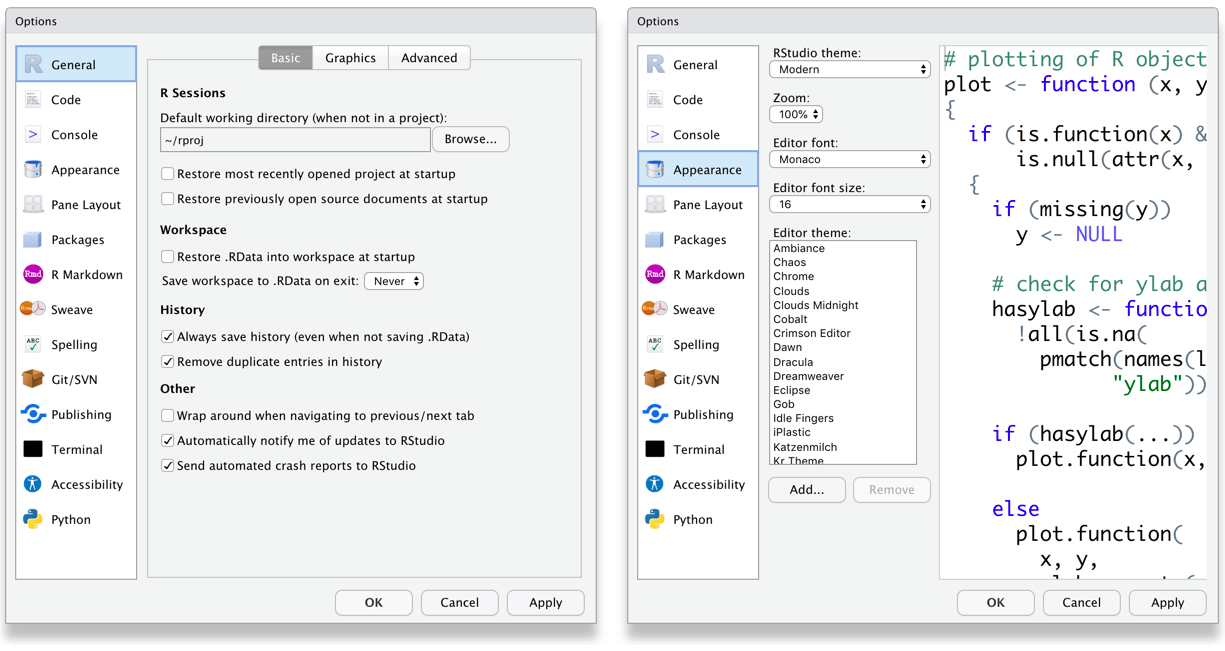
\includegraphics[width=1\linewidth]{images/rstudio_settings_general_appearance} 

}

\caption{RStudio General and Appearance settings}\label{fig:settings-general}
\end{figure}

You may also want to change the settings in the Code tab. Foe example, Lisa prefers two spaces instead of tabs for my code and likes to be able to see the whitespace characters. But these are all a matter of personal preference.

\begin{figure}

{\centering 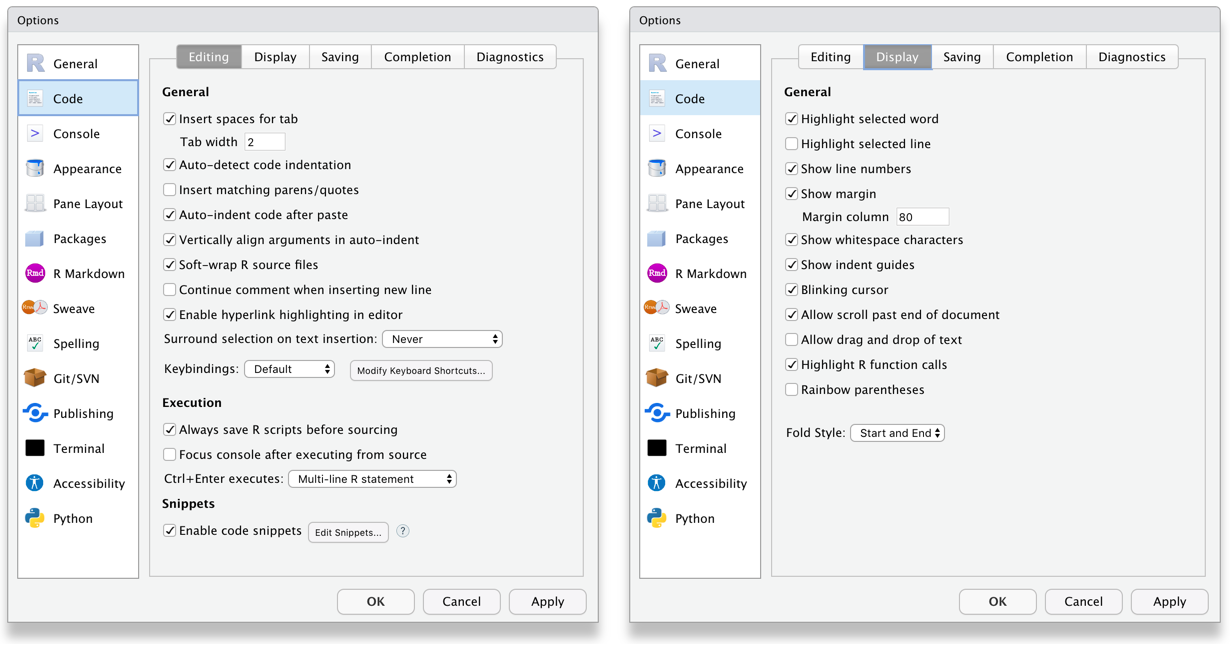
\includegraphics[width=1\linewidth]{images/rstudio_settings_code} 

}

\caption{RStudio Code settings}\label{fig:settings-code}
\end{figure}

\hypertarget{installing-latex}{%
\section{Installing LaTeX}\label{installing-latex}}

You can install the LaTeX typesetting system to produce PDF reports from RStudio. Without this additional installation, you will be able to produce reports in HTML but not PDF. This course will not require you to make PDFs. To generate PDF reports, you will additionally need to install tinytex \citep{R-tinytex} and run the following code:

\begin{Shaded}
\begin{Highlighting}[]
\NormalTok{tinytex}\SpecialCharTok{::}\FunctionTok{install\_tinytex}\NormalTok{()}
\end{Highlighting}
\end{Shaded}

\hypertarget{symbols}{%
\chapter{Symbols}\label{symbols}}

\begin{longtable}[]{@{}cll@{}}
\toprule
Symbol & psyTeachR Term & Also Known As \\
\midrule
\endhead
() & (round) brackets & parentheses \\
{[}{]} & square brackets & brackets \\
\{\} & curly brackets & squiggly brackets \\
\textless\textgreater{} & chevrons & angled brackets / guillemets \\
\textless{} & less than & \\
\textgreater{} & greater than & \\
\& & ampersand & ``and'' symbol \\
\# & hash & pound / octothorpe \\
/ & slash & forward slash \\
\textbackslash{} & backslash & \\
- & dash & hyphen / minus \\
\_ & underscore & \\
* & asterisk & star \\
\^{} & caret & power symbol \\
\textasciitilde{} & tilde & twiddle / squiggle \\
= & equal sign & \\
== & double equal sign & \\
. & full stop & period / point \\
! & exclamation mark & bang / not \\
? & question mark & \\
' & single quote & quote / apostrophe \\
" & double quote & quote \\
\%\textgreater\% & pipe & magrittr pipe \\
\textbar{} & vertical bar & pipe \\
, & comma & \\
; & semi-colon & \\
: & colon & \\
@ & ``at'' symbol & \href{https://www.theguardian.com/notesandqueries/query/0,5753,-1773,00.html}{various hilarious regional terms} \\
\ldots{} & \texttt{glossary("ellipsis")} & dots \\
\bottomrule
\end{longtable}

\begin{figure}

{\centering 
\includegraphics[width=1\linewidth]{images/soundimals_hash} 

}

\caption{[Image by James Chapman/Soundimals](https://soundimals.tumblr.com/post/167354564886/chapmangamo-the-symbol-has-too-many-names)}\label{fig:img-soundimals-hash}
\end{figure}

\hypertarget{conventions}{%
\chapter{Conventions}\label{conventions}}

This book will use the following conventions:

\begin{itemize}
\tightlist
\item
  Generic code: \texttt{list(number\ =\ 1,\ letter\ =\ "A")}
\item
  Highlighted code: {dplyr}{::}{slice\_max}{(}{)}
\item
  File paths: data/sales.csv
\item
  R Packages: tidyverse
\item
  Functions: {paste}{(}{)}
\item
  Strings: {``psyTeachR''}
\item
  Numbers: {100}, {3.14}
\item
  Logical values: {TRUE}, {FALSE}
\item
  Glossary items: ordinal
\item
  Citations: \citet{R-tidyverse}
\item
  Internal links: Chapter~\ref{foreword}
\item
  External links: \href{https://r4ds.had.co.nz/}{R for Data Science}
\item
  Menu/interface options: \textbf{\texttt{New\ File...}}
\end{itemize}

\hypertarget{webexercises}{%
\section{Webexercises}\label{webexercises}}

\begin{itemize}
\tightlist
\item
  Type an integer:
\item
  I am going to learn a lot: TRUE FALSE
\item
  What is a p-value?

  \hypertarget{radio_WPOWPLZBTY}{}
  {the probability that the null hypothesis is true} {the probability of the observed (or more extreme) data, under the assumption that the null-hypothesis is true} {the probability of making an error in your conclusion}
\end{itemize}

Hidden Text

You found some hidden text!

Hidden Code

\begin{Shaded}
\begin{Highlighting}[]
\FunctionTok{print}\NormalTok{(}\StringTok{"You found some hidden code!"}\NormalTok{)}
\end{Highlighting}
\end{Shaded}

\begin{verbatim}
## [1] "You found some hidden code!"
\end{verbatim}

\hypertarget{alert-boxes}{%
\section{Alert boxes}\label{alert-boxes}}

\begin{info}
Informational asides.

\end{info}

\begin{warning}
Notes to warn you about something.

\end{warning}

\begin{dangerous}
Notes about things that could cause serious errors.

\end{dangerous}

\begin{try}
Try it yourself.

\end{try}

\hypertarget{code-chunks}{%
\section{Code Chunks}\label{code-chunks}}

\begin{Shaded}
\begin{Highlighting}[]
\CommentTok{\# code chunks}
\FunctionTok{paste}\NormalTok{(}\StringTok{"Applied"}\NormalTok{, }\StringTok{"Data"}\NormalTok{, }\StringTok{"Skills"}\NormalTok{, }\DecValTok{1}\NormalTok{, }\AttributeTok{sep =} \StringTok{" "}\NormalTok{)}
\end{Highlighting}
\end{Shaded}

\begin{verbatim}
## [1] "Applied Data Skills 1"
\end{verbatim}

\begin{Shaded}
\begin{Highlighting}[]
\CommentTok{\# code chunks with visible r headers}
\FunctionTok{library}\NormalTok{(tidyverse)}
\end{Highlighting}
\end{Shaded}

\hypertarget{glossary}{%
\section{Glossary}\label{glossary}}

term

definition

ordinal

Discrete variables that have an inherent order, such as number of legs

\hypertarget{license}{%
\chapter*{License}\label{license}}
\addcontentsline{toc}{chapter}{License}

This book is licensed under Creative Commons Attribution-ShareAlike 4.0 International License \href{https://creativecommons.org/licenses/by-sa/4.0/}{(CC-BY-SA 4.0)}. You are free to share and adapt this book. You must give appropriate credit, provide a link to the license, and indicate if changes were made. If you adapt the material, you must distribute your contributions under the same license as the original.

  \bibliography{book.bib,packages.bib}

\end{document}
